\zotelo{../thesis.bib}

\chapter{Particle-in-Cell Method}
\label{chap:pic}

\section{Introduction}
\label{sec:introduction}

The Particle-in-Cell (PIC) technique is a powerful tool to study the kinetic
properties of plasma from first principles. The strength of a PIC code is that
it can resolve the plasma skin depth, faithfully reproducing the microscopic
interaction between particles and fields, making them invaluable in the study of
particle acceleration processes in plasmas. Also it is relatively
straight-forward to implement and easily parallelizable. It has been very
successfully applied to collisionless shocks and reconnection processes in
astrophysics
%% TODO: references
. However, because a PIC code has to resolve the
plasma skin depth which is usually many orders of magnitude smaller than the
scale of a realistic astrophysical problem, this kind of simulation is extremely
expensive and very often only applicable to local problems to study the
microphysics in a relatively large system.

This chapter introduces the PIC technique in detail, and then introduces
Aperture, a versatile PIC code designed and developed from scratch as part of my
PhD thesis. The original and main purpose of the code was to simulate the global
structure of the pulsar magnetosphere from first principles. However, we
designed the code to be general enough to be applied to many different problems
in Astrophysics, especially in problems where particles are accelerated in
strong magnetic fields and capable of producing pair cascade.

% TODO: Update this paragraph
In Section \ref{sec:particle-cell-method} we will present the numerical
algorithms and techniques employed in PIC codes, including the standard Yee
staggered grid, Boris and Vay pusher, and charge conserving current deposition.
We will also explain some of the novel features of the Aperture code, including
the treatment of general curvilinear coordinate systems, boundary conditions,
and radiative processes. Section \ref{sec:code-aperture} gives a general
overview of the Aperture code, including its architecture and highlighting some
implementation details. Section \ref{sec:test-problems} presents some test cases
to demonstrate the validity of the code. Finally Section
\ref{sec:code-discussions} discusses the strengths and weaknesses of the code,
and remark on the outstanding challenges and potential future applications.

\section{The Particle-in-Cell Method}
\label{sec:particle-cell-method}
% This section is the meat of this paper. There will probably be many
% subsections.
The PIC method is essentially a way to solve the coupled Maxwell-Vlasov
equations by approximating the plasma distribution function using the sum of a
large number of discrete macro-particle distributions, each resembling a
physical particle. The system of equations under question is simply the Maxwell
equations combined with the Vlasov equation:
\begin{align}
  \frac{\partial f^{s}}{\partial t} + \mathbf{u}\cdot\frac{\partial f^s}{\partial \mathbf{x}} &+ \frac{q^s}{m^s}\left(\mathbf{E} + \frac{\mathbf{u}}{c}\times \mathbf{B}\right)\cdot\frac{\partial f^s}{\partial (\gamma \mathbf{u})} = 0 \label{eq:vlasov}\\
  \nabla\cdot \mathbf{E} &= 4\pi\rho \\
  \nabla\cdot \mathbf{B} &= 0 \\
  \nabla\times \mathbf{E} &= -\frac{1}{c}\partial_t \mathbf{B} \\
  \nabla\times \mathbf{B} &= \frac{1}{c}\partial_t \mathbf{E} + \frac{4\pi}{c} \mathbf{j}
\end{align}
where $s$ denotes the particle species (electrons, positrons, ions,
\dots). We assume a collisionless plasma by setting the right hand
side of equation \eqref{eq:vlasov} to zero, which is applicable for many
astrophysical applications including collisionless shock acceleration,
magnetic reconnection, and pulsar wind nebulae. In these astrophysical systems
the effective free path of electrons and positrons are much larger than the
size of the system itself, rendering the collision term negligible. All plasma
interactions are mediated by the electromagnetic field.

The charge and current densities appearing in the Maxwell equations as source
terms are found by taking the moments of the distribution function $f^s$ over
the momentum space
\begin{align}
  \rho &= \int d \mathbf{u} \sum_s q^s f^s(\mathbf{x}, \mathbf{u}) \label{eqn:pic-rho} \\
  \mathbf{j} &= \int d \mathbf{u} \sum_s q^s \mathbf{u} f^s(\mathbf{x}, \mathbf{u}) \label{eqn:pic-j}
\end{align}
Macro particles are introduced to sample the distribution function $f^s$ in both
position and momentum space. We approximate the distribution function of each
species by sampling it with a finite but large number of macro particles each
with a smeared out distribution in space but unique momentum $\mathbf{p}_{p}$:
\begin{equation}
  \label{eq:single-particle}
  f^s(\mathbf{x}, \mathbf{u}) = \sum_{p}f^s_{p}(\mathbf{x}, \mathbf{u}) = \sum_{p}\delta(\gamma m_{p}\mathbf{u} - \mathbf{p}_{p}) \mathcal{S}(\mathbf{x} - \mathbf{x}_{p})
\end{equation}
% A macro particle can be
% viewed as a collection of particles smeared out in space, with
% identical physical momentum $\mathbf{p}_{p}$. Therefore, each
% particle represents a distribution function of the type
where $\mathcal{S}$ is a function that describes the shape of the macro particle, with the
property that $\mathcal{S}$ has finite support, and that the integral of $\mathcal{S}$ over all
space is normalized to 1. Since the Vlasov equation is linear, if each
individual macro particle satisfies the Vlasov equation, then the linear
superposition of a large number of them still satisfy the Vlasov equation, and
should provide a good approximation for the dynamics of the plasma.

The dynamic equations for the macro particles can be derived by taking
the moments of the Vlasov equation with the single particle
distribution function \eqref{eq:single-particle}. Plugging the single
particle distribution function into the Vlasov equation and taking the
zeroth moment by integrating over $\mathbf{u}$, we get
\begin{equation}
  \begin{split}
    \int d\mathbf{u}\,\left\{ \left[ \partial_t \delta(\gamma m_{p}\mathbf{u} - \mathbf{p}_p) \right]\mathcal{S}(\mathbf{x} - \mathbf{x}_p) + \delta(\gamma m_{p}\mathbf{u} - \mathbf{p}_p)\partial_t\mathcal{S}(\mathbf{x} - \mathbf{x}_p) \right. \\
    + \delta(\gamma m_{p}\mathbf{u} - \mathbf{p}_p) \mathbf{u}\cdot\nabla \mathcal{S}(\mathbf{x} - \mathbf{x}_p) \\
    \left. + \mathcal{S}(\mathbf{x} - \mathbf{x}_p)\frac{q_p}{m_p}\left(\mathbf{E} +
        \frac{\mathbf{u}}{c}\times \mathbf{B}\right)\cdot \nabla_{\gamma
        \mathbf{u}}\delta(\gamma m_{p}\mathbf{u} - \mathbf{p}_p) \right\} = 0
  \end{split}
\end{equation}
The first term is an integral of the derivative of a delta function,
which should give zero since $\mathcal{S}$ is independent of the integration variable $\mathbf{u}$. The
second and third term can be integrated trivially to get
\begin{equation}
  \label{eq:eom-position}
\frac{d\mathbf{x}_p}{dt} = \mathbf{u}_p = \frac{\mathbf{p}_p}{\gamma_p m_{p}}
\end{equation}
since $\mathbf{x}_p$ depends only on $t$, the partial derivative becomes a total
derivative, $\partial_t\mathcal{S}(\mathbf{x} - \mathbf{x}_p) = -\nabla \mathcal{S}(\mathbf{x} -
\mathbf{x}_p) \cdot d\mathbf{x}_p/dt$. The last term which involves the
electromagnetic force requires a bit more attention. The $\mathbf{E}$ field term
again integrates to zero since it is an integral of the derivative of a delta
function. The Lorentz force term needs an integration by parts, but then it
would become zero because $\nabla_{\gamma \mathbf{u}}\cdot(\mathbf{u}\times
\mathbf{B})$ is zero.

% The dynamic equations for the macro particles can be derived by taking
% the moments of the Vlasov equation with the single particle
% distribution function \eqref{eq:single-particle}. It turns out that
% these dynamic equations are identical to the equations of motion of a
% single particle in electromagnetic field:
% \begin{align}
%   \label{eq:particle-equations}
%   \frac{d\mathbf{x}_p}{dt} = \mathbf{u}_p = \frac{\mathbf{p}_p}{\gamma_p} \\
%   \frac{d\mathbf{p}_p}{dt} = \frac{q_p}{m_p}(\mathbf{E} + \mathbf{u}_p\times \mathbf{B})
% \end{align}
% Therefore it is justified to treat macro particles as their name
% suggests: simply as physical particles. The code simply trace their
% motion in the electromagnetic field as described by the above dynamic
% equations.

Taking the first moment of the Vlasov equation yields
\begin{equation}
\begin{split}
    \int d\mathbf{u}\,\left\{ \mathbf{u}\left[ \partial_t \delta(\gamma m_{p}\mathbf{u} - \mathbf{p}_p) \right]\mathcal{S}(\mathbf{x} - \mathbf{x}_p) + \mathbf{u}\delta(\gamma m_{p}\mathbf{u} - \mathbf{p}_p)\partial_t\mathcal{S}(\mathbf{x} - \mathbf{x}_p) \right. \\
    + \mathbf{u}\delta(\gamma m_{p}\mathbf{u} - \mathbf{p}_p) \mathbf{u}\cdot\nabla \mathcal{S}(\mathbf{x} - \mathbf{x}_p) \\
    \left. + \mathbf{u}\mathcal{S}(\mathbf{x} - \mathbf{x}_p)\frac{q_p}{m_p}\left(\mathbf{E} + \frac{\mathbf{u}}{c}\times \mathbf{B}\right)\cdot \nabla_{\gamma \mathbf{u}}\delta(\gamma m_{p}\mathbf{u} - \mathbf{p}_p) \right\} = 0
\end{split}
\end{equation}
The second and third terms give the same equation of motion as above, and they
are proportional to the gradient of $\mathcal{S}$, independent of the other two terms,
therefore we ignore them. The last two terms can be reduced to the simple
single-particle equation of motion:
\begin{equation}
  \label{eq:eom-momentum}
\frac{d\mathbf{p}_p}{dt} = q_p\left(\mathbf{E} + \frac{\mathbf{u}_{p}}{c}\times \mathbf{B} \right)
\end{equation}

These are simply equations of motion for ordinary particles in an
electromagnetic field. Therefore it is justified to treat macro particles as
their name suggests: simply as physical particles. A PIC code simply traces their
motion in the electromagnetic field as described by the above dynamic equations.


\subsection{Discretization and Spatial Grid}
\label{sec:discretization}

So far the only approximation we have introduced is using an ensemble of macro
particles to approximate the real distribution function of a plasma system. To
solve the Maxwell equations and particle dynamic equations numerically, one
needs to discretize the continuous field quantities onto a finite grid
consisting of cells, hence the name Particle-in-Cell. The discretization is done
on space and time using the Finite Difference Time Domain (FDTD)
method. %TODO: Reference?
Fields $\mathbf{E}$ and $\mathbf{B}$ are sampled on a finite grid, as well as
the current and charge densities $\mathbf{J}$ and $\rho$. One evolves the
equations using a given time evolution scheme step by step starting from the
initial condition. At each step, one updates the positions and momenta of all
particles according to the fields on the grid, computes the current density due
to particle motion, and uses this current density to evolve the fields
themselves.

A PIC code can operate in either 2D or 3D\footnote{In 1D, a discretization is
  not necessary, since there is no magnetic field, and electric field at any
  given particle location can be found exactly by integrating Gauss's law. See
  chapter \ref{chap:polar-cap}.}.
In the former case, although a grid of lower dimension is used, all 3 vector
components of $\mathbf{E}$ and $\mathbf{B}$ fields need to be
evolved\footnote{A code like this is sometimes called ``2.5D'' due to full 3D vector quantities
  defined on a 2D grid.}. This is applicable when the problem has inherent
symmetry, such as axisymmetry or translational invariance in one direction. It
is typical to use the classical staggered \citet{yee_numerical_1966} grid for
electric and magnetic fields (figures \ref{fig:Yee} and
\ref{fig:Yee-cartesian}).

\begin{figure}[h]
  \centering
  \begin{tikzpicture}[label distance=-2.5mm]
    \begin{scope}[scale=1.3]
      \draw[->] (-0.5, 0) -- node[left] {$r$} (-0.5, 2);
      \draw[->] (0, -0.5) -- node[below] {$\theta$} (2, -0.5);
      \draw[dashed] (0,0) rectangle (3,3);
      \node [label=below:$\rho\text{, }j_{\phi}\text{, }E_{\phi}$] (center) at (1.5,1.5) {$\times$};
      \node [label=right:$j_{\theta}\text{, }E_\theta\text{, }B_{r}$] (right) at (3,1.5) {$\times$};
      \node [label=above:$j_r\text{, }E_r\text{, }B_{\theta}$] (top) at (1.5,3) {$\times$};
      \node [label=right:$B_\phi$] (top right) at (3,3) {$\times$};
    \end{scope}
  \end{tikzpicture}
  \caption{Staggered Yee cell for a 2D spherical grid.}
  \label{fig:Yee}
\end{figure}

\begin{figure}[h]
  \centering
  \begin{tikzpicture}[label distance=-2.5mm]
    \begin{scope}[scale=1]
      \pgfmathsetmacro{\l}{4}
      \pgfmathsetmacro{\h}{2}
      \pgfmathsetmacro{\d}{0.8}
      \draw[dashed] (0, 0, 0) -- ++(\l, 0, 0);
      \draw[dashed] (0, 0, 0) -- ++(0, \l, 0);
      \draw[dashed] (0, 0, 0) -- ++(0, 0, \l);
      \draw[thin] (0, 0, \l) -- ++(\l, 0, 0) -- ++(0, 0, -\l)
      -- ++(0, \l, 0) -- ++(-\l, 0, 0) -- ++(0, 0, \l) -- cycle;
      \draw[thin] (\l, \l, \l) -- ++(-\l, 0, 0);
      \draw[thin] (\l, \l, \l) -- ++(0, -\l, 0);
      \draw[thin] (\l, \l, \l) -- ++(0, 0, -\l);
      \draw[very thick, ->, red] (\h, \l, \h) node[right] {$j_z,\ E_z$} -- ++(0, \d, 0);
      \draw[very thick, ->, red] (\h, \h, \l) -- ++(0, 0, \d) node[below] {$j_x,\ E_x$};
      \draw[very thick, ->, red] (\l, \h, \h) node[below] {$j_y,\ E_y$} -- ++(\d, 0, 0);
      \draw[very thick, ->, blue] (0, \h, \l) node[left] {$B_z$} -- ++(0, \d, 0);
      \draw[very thick, ->, blue] (\h, 0, \l) node[below] {$B_y$} -- ++(\d, 0, 0);
      \draw[very thick, ->, blue] (\l, 0, \h) node[below right] {$B_x$} -- ++(0, 0, \d);
      \node[label=below left:$\rho$] at (0, 0, \l) {};

      \draw[->] (-3, -3, 0) -- (1, -3, 0) node[below] {$y$};
      \draw[->] (-3, -3, 0) -- (-3, 1.2, 0) node[left] {$z$};
      \draw[->] (-3, -3, 0) -- (-3, -3, 3) node[above left] {$x$};
      % \draw (0,0,0) rectangle (3,0,3);
      % \draw (0,0,0) rectangle (0,3,3);
      % \node [label=below:$\rho\text{, }j_{\phi}\text{, }E_{\phi}$] (center) at (1.5,1.5) {$\times$};
      % \node [label=right:$j_{\theta}\text{, }E_\theta\text{, }B_{r}$] (right) at (3,1.5) {$\times$};
      % \node [label=above:$j_r\text{, }E_r\text{, }B_{\theta}$] (top) at (1.5,3) {$\times$};
      % \node [label=right:$B_\phi$] (top right) at (3,3) {$\times$};
    \end{scope}
  \end{tikzpicture}
  \caption{Staggered Yee cell for a 3D Cartesian grid.}
  \label{fig:Yee-cartesian}
\end{figure}

The reason for staggering the fields this way is that all numerical derivatives
that arise in Maxwell equations will be centered naturally and have at least
second order accuracy. For example take the evolution of the $B_z$ term:
\begin{equation}
  % \label{eq:2}
  \begin{split}
    \frac{\Delta B_z(x, y)}{\Delta t} = -(\nabla\times \mathbf{E})_{z} = &-\left[ \frac{E_x(y + \Delta y/2) - E_x(y - \Delta y/2)}{\Delta y} \right. \\
      &- \left.\frac{E_y(x + \Delta x/2) - E_y(x - \Delta x/2)}{\Delta x} \right]
  \end{split}
\end{equation}
The electric field values needed show up exactly where they are defined on
the Yee lattice, and due to the symmetric structure of the finite difference,
the $\Delta x^{2}$ term in the Taylor expansion naturally cancels:
\begin{equation}
  \label{eq:finite-diff-2nd-order}
\partial_xE_y = \frac{E_y(x + \Delta x/2) - E_y(x - \Delta x/2)}{\Delta x} + \mathcal{O}(\Delta x^3)
\end{equation}
This naturally applies to all derivative terms in the Maxwell equation.

Another strength of the Yee grid is that the differential relations
$\nabla\cdot(\nabla\times \mathbf{F}) = 0$ and $\nabla \times \nabla f = 0$ are
satisfied by construction, so long as Maxwell equations are used for the
evolution of fields, $\nabla\cdot \mathbf{B} = 0$ should be preserved to
numerical precision without extra work.

This construction of symmetric finite difference scheme allows the extension to
higher orders naturally. Equation \eqref{eq:finite-diff-2nd-order} is accurate
to second order in $\Delta x$. To achieve 4th order accuracy, we need to use
more terms to cancel out the $\Delta x^{3}$ term in the Taylor expansion:
% TODO: Fix this expression
\begin{equation}
  \label{eq:finite-diff-4th-order}
  \partial_{x}E_y = \frac{9}{8}\frac{E_y(x + \Delta x/2) - E_y(x - \Delta x / 2)}{\Delta x} - \frac{1}{24}\frac{E_y(x + 3\Delta x / 2) - E_y(x - 3\Delta x / 2)}{\Delta x} + O(\Delta x^5)
\end{equation}
Further discussion of the implementation of higher order finite difference
schemes can be found in appendix \ref{app:finite-diff}.

Macro-particles stream freely in the grid, and their positions and momenta are
not discretized. To convert between local ``particle'' quantities and grid
variables, an interpolation scheme is required. Fortunately we already have a
function $\mathcal{S}(\mathbf{x} - \mathbf{x}_p)$ which describes the shape of
the macro particle smeared in space. Integrating equation \eqref{eqn:pic-rho}
using a macro particle distribution function over the volume of a cell gives:
\begin{equation}
  \label{eqn:rho-cell}
  Q_{c} = \rho_{c}\Delta V = \sum_pq_pS(\mathbf{x}_p-\mathbf{x}_{c})
\end{equation}
where $q_p$ is the charge of an individual macro particle, $\mathbf{x}_{c}$ is
the position of the center of the cell, and $S$ is defined as
the integral of $\mathcal{S}$:
\begin{equation}
  \label{eqn:weight-function}
  S(\mathbf{x}_p - \mathbf{x}_c) = \int_{\mathbf{x}_c - \bm{\Delta}/2}^{\mathbf{x}_c + \bm{\Delta}/2} \mathcal{S}(\mathbf{x}_p - \mathbf{x})d\mathbf{x}
\end{equation}
and $\bm{\Delta}$ is the size of the cell. The assumption that $\mathcal{S}$ has
finite support implies that $S$ will be nonzero for only a few cells with
$\mathbf{x}_{c}$ close to $\mathbf{x}_{p}$, and since the integration of
$\mathcal{S}$ over the whole volume is constrained to be 1, the sum of all
nonzero $S$ near a certain particle is guaranteed to be 1. This is another way
of saying total charge is conserved. Since in the PIC code we will only be
using the discrete interpolation functions $S$, not the original $\mathcal{S}$,
we will call $S(\mathbf{x}_p - \mathbf{x}_c)$ the ``shape function''.
Typical shape functions used in PIC codes are derived from so-called
``B-spline'' functions, which are piecewise polynomial functions with minimal
support. Following are the shape functions often used in PIC codes, in ascending
polynomial order:

\textbf{CIC}: Cloud in Cell
\begin{equation}
  \label{eq:first-order-deposit}
  S^1(x) = \begin{cases}
    \displaystyle 1 - |\delta| & \quad \text{if } |\delta| < 1, \\
    \displaystyle 0            & \quad \text{otherwise}
  \end{cases}
\end{equation}

\textbf{TSC}: Triangular Shaped Cloud
\begin{equation}
  \label{eq:second-order-deposit}
  S^2(x) =
  \begin{cases}
    \displaystyle \frac{3}{4} - \delta^2 & \quad \text{if } |\delta| < 1/2, \\
    \displaystyle \frac{1}{2} \left( \frac{3}{2} - |\delta| \right)^2 & \quad \text{if } 1/2 \leq |\delta| < 3/2, \\
    \displaystyle 0                      & \quad \text{otherwise}
  \end{cases}
\end{equation}

\textbf{PCS}: Piecewise Cubic Spline
\begin{equation}
  \label{eq:third-order-deposit}
  S^3(x) =
  \begin{cases}
    \displaystyle \frac{1}{6} \left( 4 - 6\delta^2 + 3|\delta|^3 \right) & \quad \text{if } |\delta| < 1, \\
    \displaystyle \frac{1}{6} \left( 2 - |\delta| \right)^3 & \quad \text{if } 1 \leq |\delta| < 2, \\
    \displaystyle 0                      & \quad \text{otherwise}
  \end{cases}
\end{equation}

These functions are the integration of the B-spline functions of the
corresponding polynomial order \citep{haugboelle_photon-plasma:_2012}.
% TODO: insert a plot of these functions
In 2D or 3D problems, the weight of the particle is given by multiplication of
these shape functions, e.g.\ in 3D Cartesian coordinates $S(\mathbf{x}_{p} -
\mathbf{x}_{c}) = S(x_{p} - x_{c})S(y_{p} - y_{c})S(z_{p} - z_{c})$. In general,
higher order shape functions will have better noise properties for the result,
but are computationally more intensive, not only because they involve more
multiplications (higher order polynomial), but each particle can influence more
grid points and one needs to sum over more terms of nonzero $S$.

Equation \eqref{eqn:rho-cell} can be taken as the definition of the discretized
charge density in a given cell. In other words, it is the average charge
contained in the cell assuming the cell is uniformly filled with charges from
the macro particles.

The particle shape function also serves as a way to interpolate the grid
quantities such as $\mathbf{E}$ and $\mathbf{B}$ fields to the particle
location:
\begin{align}
    \label{eqn:interpolate}
    \mathbf{E}(\mathbf{x}_p) &= \sum_c \mathbf{E}(\mathbf{x}_c) S(\mathbf{x}_p - \mathbf{x}_c) \\
    \mathbf{B}(\mathbf{x}_p) &= \sum_c \mathbf{B}(\mathbf{x}_c) S(\mathbf{x}_p - \mathbf{x}_c)
\end{align}
where the summation is over the grid points where $S \neq 0$.

One could also define and compute the current density in the same way as charge density,
from equation \eqref{eqn:pic-j}:
\begin{equation}
  \label{eq:naive-j}
  \mathbf{j} ( \mathbf{x}_{c} ) = \sum_{p} \frac{q_{p}}{\Delta V}\mathbf{u}_p S (
  \mathbf{x}_{p} -\mathbf{x}_{c} )
\end{equation}
However, simple application of this equation will lead to charge
conservation issues and violation of the continuity equation \citetext{see e.g.\
  \citealp{hockney_computer_1981}, \citealp{birdsall_plasma_1991}}
%% TODO: Finish citation
\begin{equation}
    \label{eq:continuity}
    \partial_t\rho + \nabla\cdot \mathbf{j} = 0
\end{equation}

To enforce charge conservation at every timestep, instead of interpolating on
the current, it is desirable to solve the continuity equation directly at every
timestep. This is done with the so-called charge-conserving current deposition.
We will discuss various techniques to achieve this in section
\ref{sec:charge-cons-curr}.


% Since particles stream freely in the cells, the electric and magnetic
% fields a particle sees will need to be interpolated from the grid
% points. This is done by integrating the shape function in equation
% \eqref{eq:single-particle}:
% \begin{equation}
%     \label{eq:field-interpolate}
%     \mathbf{E}_p = \int d\mathbf{x}\: S(\mathbf{x} - \mathbf{x}_p)\mathbf{E}(\mathbf{x}) = \sum_c W(\mathbf{x}_c - \mathbf{x}_p)E_c
% \end{equation}
% where the subscript $c$ runs over all grid points. The function $W$ is
% a weight function which has finite support centered around
% $\mathbf{x}_p$ and sums to 1 on grid points where it does not
% vanish. They are often chosen to be the so called \textit{B-spline}
% functions, which are functions of minimal support with a given
% polynomial degree. Higher order polynomial B-splines will in general
% produce a smoother interpolation, but will be more computationally
% expensive. In Aperture we support weight functions from 0-th order to
% 3-rd order polynomials.

% Conversely, particle motion is interpolated onto the grid to produce a
% current and charge density. To avoid spurious self-force, one needs to
% use the same interpolation for both field to particle, and for
% particle to current. We will discuss current deposition in greater
% detail in section \ref{sec:charge-cons-curr}.

\subsection{Current Deposition}
\label{sec:charge-cons-curr}

There are various ways to achieve charge conservation numerically. The simplest
way is to use the naive current deposition \eqref{eq:naive-j}, being aware of
the fact that it does not conserve charge according to the continuity equation.
As a result, $\nabla\cdot \mathbf{E}/4\pi$ will slowly deviate from the charge
density $\rho$. This will turn up in the simulation as artifacts in the electric
field as if there is spurious charge density dispersed in the plasma
distribution which are not tracked by the code. Depending on the application,
this might or might not be an issue, and some PIC codes decide to ignore this
problem in favor of faster computation speed.

A typical way to help alleviate this problem is to employ divergence
cleaning. There is no unique way of doing this, and many methods exist in
literature.  % TODO: references
We only outline a simple method here. The goal is to solve the equation
$\nabla\cdot \mathbf{E} = 4\pi\rho$ every few timesteps. Since the deviation
built up over a short time should be small as long as the time step is small,
one can solve a diffusion equation of the electric potential $\phi$
\begin{equation}
  \label{eq:diffusion-electric-potential}
  \frac{\partial\phi}{\partial t} = -\nabla^2\phi - 4\pi\rho
\end{equation}
Since the diffusion equation has the property that an initial distribution with
nonzero right hand side will relax towards an equilibrium where the right hand
side becomes zero, we only need to apply some relaxation iterations to let it
converge. A typical method is the Gauss-Seidel method \citep[see
e.g.][]{press_numerical_2007} which applies a filter to the field consecutively.
Since the initial deviation should be small, it only takes several relaxation
iterations to achieve a reasonable result.

One difficulty of divergence cleaning lies in parallelization, since the
relaxation filter is usually a global operation which involves communication
between nodes every time (see section \ref{sec:code-aperture} for
parallelization). Another problem is that it inevitably introduces tiny
fluctuations to the electric field, which will couple to particle dynamics and
introduce heating to the plasma. A more efficient way is to directly solve the
continuity equation \eqref{eq:continuity} for $\mathbf{j}$ at every timestep,
which ensures that it is satisfied to numerical precision. Since charge density
$\rho$ never really shows up in the evolution equations in the first place, it
only serves as a constraint for electric field, therefore we can actually avoid
evaluating the charge density and deposit $\mathbf{j}$ directly. As long as the
condition $\nabla\cdot \mathbf{E} = 4\pi\rho$ is satisfied for the initial
condition, the continuity equation will guarantee that it is satisfied in
subsequent times to numerical precision, thus side-stepping the problem of
charge-conservation.

There are two main ways to solve the continuity equation numerically at each
timestep. The classical way was proposed by \citet{villasenor_rigorous_1992},
which uses exact solutions for charge fluxes across cell boundaries for each
kind of particle movement pattern. The Buneman deposit assumes first order shape
functions (equation \eqref{eq:first-order-deposit}), and particles are effectively
squares (cubes in 3D). When particles move, their shapes will overlap with some
cell boundaries, creating charge fluxes across these boundaries and thus
creating current. It is possible to solve exactly for the amount of current
induced on each cell surface, effectively solving the continuity equation to
machine precision.

\begin{figure}[h]
  \centering
  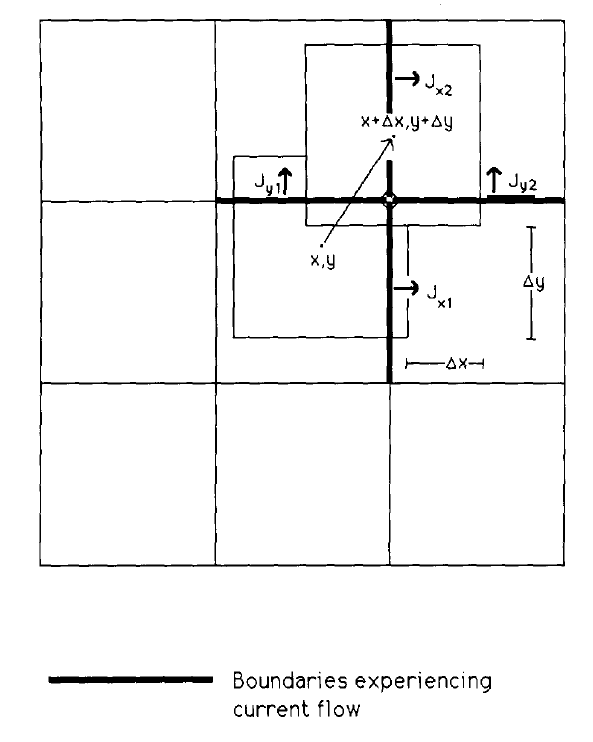
\includegraphics[width=0.32\textwidth]{pics/chap1/buneman-1.png}
  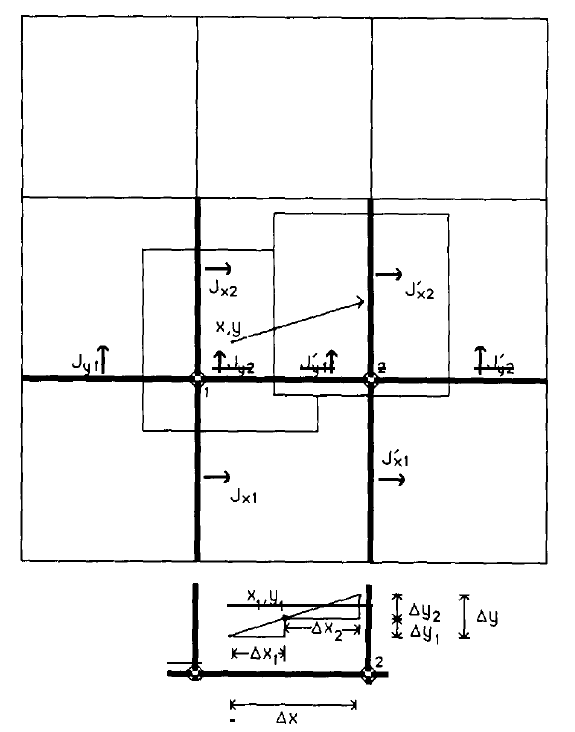
\includegraphics[width=0.32\textwidth]{pics/chap1/buneman-2.png}
  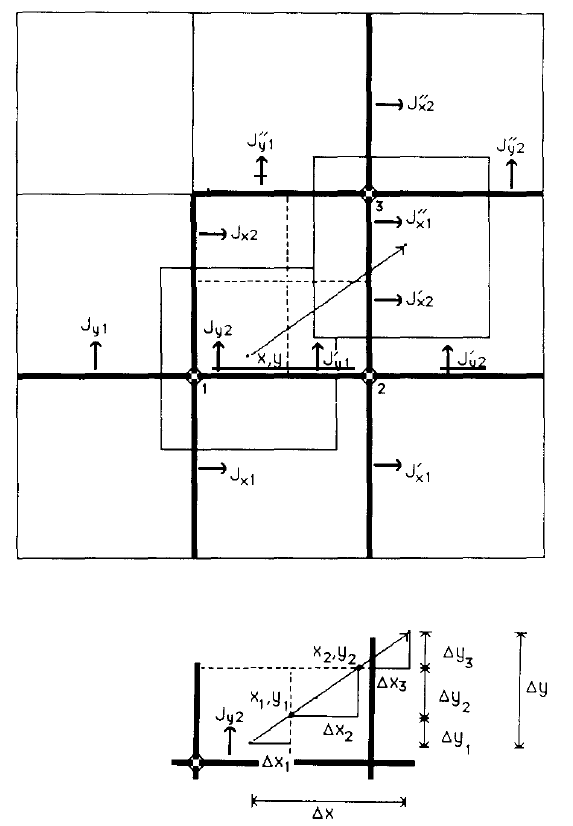
\includegraphics[width=0.32\textwidth]{pics/chap1/buneman-3.png}
  \caption[Three cases for Buneman cell crossing in 2D.]{Three cases for Buneman
    cell crossing in 2D \citep{villasenor_rigorous_1992}. The first case is the
    simplest where the particle shape only intersects with 4 boundaries during
    its movement. The second case involves 7 boundaries, and can be decomposed
    into two 4-boundary segments. The third case involves 10 boundaries and can
    be decomposed into 3 segments of 4-boundary movement.}
  \label{fig:buneman}
\end{figure}

The difficulty of this method lies in the many ways the cell boundary can be
crossed. In 2D, there are 3 different cases where the moving particle can cross
4, 7, or 10 cell boundaries in a particular timestep (figure \ref{fig:buneman}).
For the simplest case where only 4 boundaries are crossed, the current involved
can be easily found to be:
\begin{align}
  \label{eq:buneman-4-cross-a}
  J_{x1} &= q\Delta x \left( \frac{1}{2} - y - \frac{1}{2}\Delta y \right) ,\quad J_{x2} = q\Delta x \left( \frac{1}{2} + y + \frac{1}{2}\Delta y \right) \\
  \label{eq:buneman-4-cross-b}
  J_{y1} &= q\Delta y \left( \frac{1}{2} - x - \frac{1}{2}\Delta x \right) ,\quad J_{y2} = q\Delta y \left( \frac{1}{2} + x + \frac{1}{2}\Delta x \right)
\end{align}

For the 7-boundary case, it can be decomposed into 2 4-boundary moves, and
similarly the 10-boundary case can be decomposed into 3 4-boundary moves. Care
must be taken when decomposing the moves, since the second move can involve 4
different set of 4 boundaries, depending on the direction the particle moves.
After decomposing the particle path into segments, each segment is treated as an
ordinary move and equations \eqref{eq:buneman-4-cross-a} and
\eqref{eq:buneman-4-cross-b} are used for each segment. The final current due to
the complete particle path is the sum of the current from each segment.

The situation becomes worse in 3D. The simplest case involves current through 12
faces (4 faces on each coordinate plane), and the more complex cases are treated
as follows: each time the particle crosses a cell face, the displacement is
split into two segments, each consists of only movement within a single cell,
which only needs to deal with 12 faces. This involves many branching and many
if-else statements in the actual code. When implemented properly
the difference between divergence of $E$ field and the charge density stays
within truncation error of the floating point precision used in the calculation.
Note that in this algorithm, it was implicitly assumed that the particle can not
move more than one cell spacing. This condition is usually satisfied due to the
Courant condition (section \ref{sec:fd-maxwell}) being a more strict
requirement.

\begin{figure}[h]
  \centering
  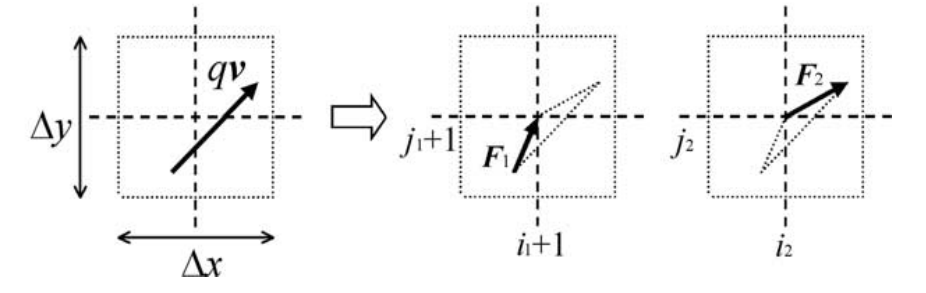
\includegraphics[width=0.6\textwidth]{pics/chap1/umeda-1.png}\\
  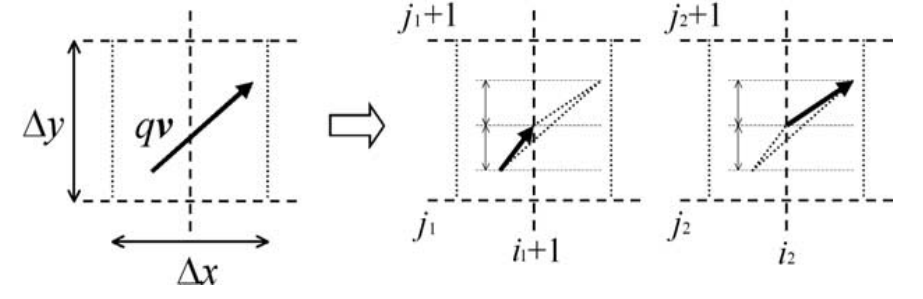
\includegraphics[width=0.6\textwidth]{pics/chap1/umeda-2.png}
  \caption[Zigzag scheme for current deposition.]{Zigzag scheme for current
    deposition. Mid points are chosen to be a cell vertex if the particle
    crosses two boundaries, or the midpoint of the cell face of perpendicular
    position on the crossed boundary if only there is only one cell crossing.
    \cite{umeda_new_2003}}
  \label{fig:zigzag-2d}
\end{figure}

This method was later improved by \citet{umeda_new_2003} to cut down the number
of different cases and increasing performance by splitting the particle path in
the case of cell-crossing into a zigzag pattern. They noticed that the branching
conditions for Buneman pusher depend mostly on whether the particle in question
crosses a cell boundary. The idea is simply to find a universal midpoint for all
kinds of trajectories to reduce the number of necessary segments to the minimum.
The cases in 2D are shown in figure \ref{fig:zigzag-2d}. This way, the particle
path in one timestep is split to at most 2 segments, saving a lot of branching
cases. Each segment is then deposited using the standard equations
\eqref{eq:buneman-4-cross-a} and \eqref{eq:buneman-4-cross-b}. The improvement
is even more significant in 3D, where again only 4 cases are needed (figure
\ref{fig:zigzag-3d}), and in all cases only up to two segments in one timestep
is needed to complete the deposition, greatly simplifying the amount of
computations needed compared to the original Buneman scheme. Another strength of
this method is that higher order shape functions \eqref{eq:second-order-deposit}
or \eqref{eq:third-order-deposit} can be used since after segmenting the
particle path, the only case one need to consider is one where particle does not
cross cell boundary, and the current due to this movement can be solved exactly,
whereas the original Buneman algorithm will need to consider many more different
cases due to one particle has influence on many more cell faces.

\begin{figure}[h]
  \centering
  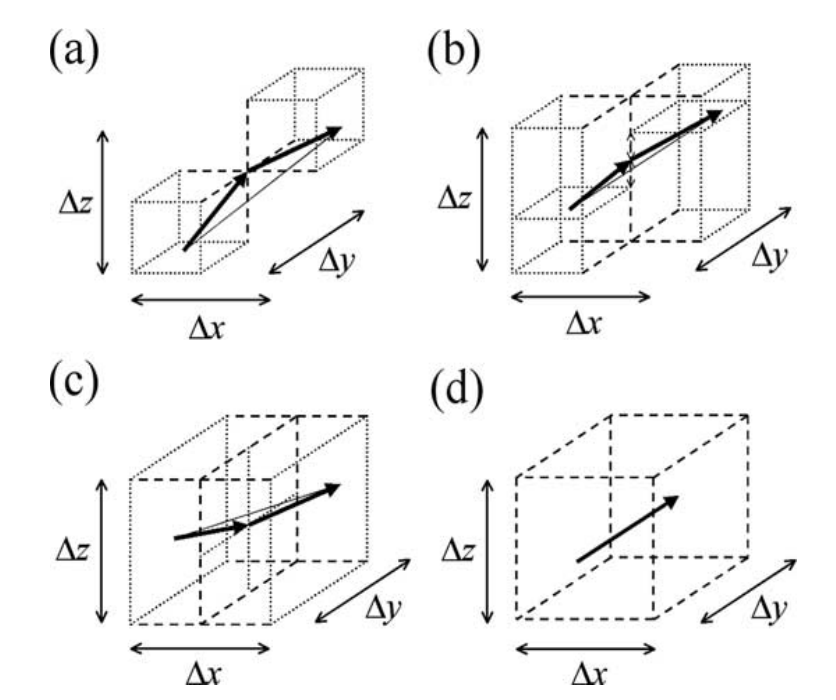
\includegraphics[width=0.6\textwidth]{pics/chap1/umeda-3d.png}
  \caption[Zigzag scheme in 3D.]{Zigzag scheme for 3D. Only up to 2 segments are
    needed for all cases of cell-crossing, reduced from the up to 8 cases of the
    original Buneman scheme, greatly reducing the number of operations. \cite{umeda_new_2003}}
  \label{fig:zigzag-3d}
\end{figure}

Another way to solve the continuity equation is proposed by
\citet{esirkepov_exact_2001}. It decomposes the motion of charged particles into
motions along individual axes since they are independent. Then the change of
charge density $\Delta\rho$ is split into components that correspond to
components of $\nabla\cdot \mathbf{j}$. This is simplest to write in
Cartesian coordinates:
\begin{equation}
  \label{eq:esirkepov-split}
  \Delta \rho = \Delta\rho_{x} + \Delta\rho_{y} + \Delta\rho_{z} = -\Delta t(\partial_{x}j_{x} + \partial_{y}j_{y} + \partial_{z}j_{z})
\end{equation}
Due to the fact that coordinate directions are independent, motion of particles
in $x$ direction for example does not generate current in the $y$ and $z$
direction. This means that we can identify the $\partial_{x}j_{x}$ term with
$\Delta \rho_{x}$, similarly for the $y$ and $z$ terms. For the simplest case
where $\partial_{x}$ is simply the 2-term symmetric finite difference operator
\ref{eq:finite-diff-2nd-order}, then we can write
\begin{equation}
  \label{eq:esirkepov-x-dir}
  j_{x}(x + \Delta x/2) = j_{x}(x - \Delta x/2) - \frac{\Delta x}{\Delta t}\Delta\rho_{x}(x)
\end{equation}
Given a boundary condition of $j$ at one boundary (usually $j = 0$), one can do
a prefix sum over $\Delta\rho$ to get the local $j_{x}$ of each cell. This may
sound like a very expensive operation, especially when parallelization is
considered, since each node down the row will need to wait for the previous node
to finish the prefix sum and take the final result to start the accumulation of
this node. However practically since all particle shape functions have finite
support, one simply needs to pass $\Delta\rho$ in the guard cells to the
neighboring nodes, then each node can start the prefix sum from $j = 0$
independently. See section \ref{sec:code-aperture} for discussion on domain
decomposition and guard cells.

Now the task is simply to find $\Delta\rho$ for each direction.
\citet{esirkepov_exact_2001} found a unique solution for them in terms of
particle shape functions $S$:
\begin{equation}
  \label{eq:esirkepov-solution}
  \begin{split}
    \frac{\Delta \rho_{x}(i, j, k)}{q} = &\frac{1}{3}S(x + \Delta x, y + \Delta y, z + \Delta z) - \frac{1}{3}S(x, y + \Delta y, z + \Delta z) \\
    &+ \frac{1}{6}S(x + \Delta x, y, z + \Delta z) - \frac{1}{6}S(x, y, z + \Delta z) \\
    &+ \frac{1}{6}S(x + \Delta x, y + \Delta y, z) - \frac{1}{6}S(x, y + \Delta y, z) \\
    &+ \frac{1}{3}S(x + \Delta x, y, z) - \frac{1}{3}S(x, y, z)
  \end{split}
\end{equation}
where $x$, $y$, $z$ are the original position of the particle, $\Delta x$,
$\Delta y$, $\Delta z$ are the particle displacements during one timestep, and
$S(x + \Delta x, y + \Delta y, z + \Delta z)$ is the shape function evaluated
for the particle at the final position, with respect to the cell for which we
are evaluating $\rho_{x}$. For other directions simply permute the coordinate
indices. Figure \ref{fig:esirkepov-average} shows a geometric interpretation of
this solution as an average over 3 parallel paths.

\begin{figure}[h]
  \centering
  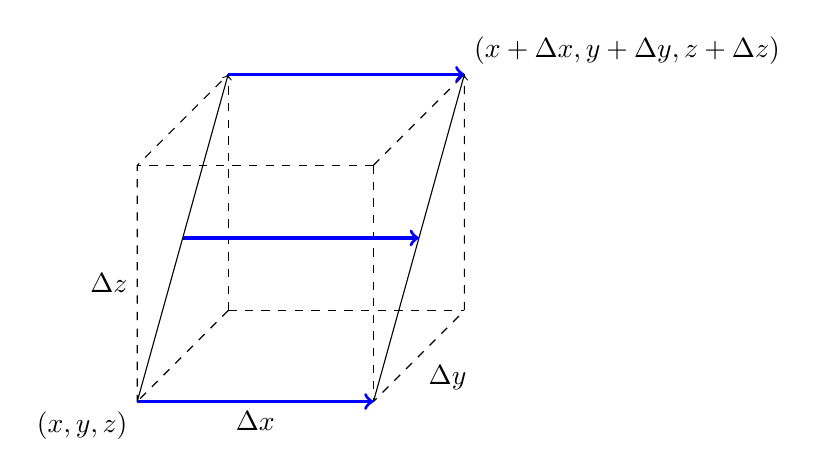
\begin{tikzpicture}
    \pgfmathsetmacro{\l}{3}
    \pgfmathsetmacro{\h}{1.5}
    \draw[dashed] (0, 0, 0) -- ++(\l, 0, 0);
    \draw[dashed] (0, 0, 0) -- ++(0, \l, 0);
    \draw[dashed] (0, 0, 0) -- ++(0, 0, \l) node[below left] {$(x, y, z)$};
    \draw[dashed] (0, 0, \l) -- node[below] {$\Delta x$} ++(\l, 0, 0) -- node[below right] {$\Delta y$} ++(0, 0, -\l) -- ++(0, \l, 0) -- ++(-\l, 0, 0) -- ++(0, 0, \l) -- node[left] {$\Delta z$} ++(0, -\l, 0);
    \draw[dashed] (\l, \l, \l) -- ++(-\l, 0, 0);
    \draw[dashed] (\l, \l, \l) -- ++(0, -\l, 0);
    \draw[dashed] (\l, \l, \l) -- ++(0, 0, -\l) node[above right] {$(x + \Delta x, y + \Delta y, z + \Delta z)$};
    \draw[->] (0, 0, \l) -- (0, \l, 0);
    \draw[->] (\l, 0, \l) -- (\l, \l, 0);
    \draw[blue,very thick,->] (0, \l, 0) -- ++(\l, 0, 0);
    \draw[blue,very thick,->] (0, 0, \l) -- ++(\l, 0, 0);
    \draw[blue,very thick,->] (0, \h, \h) -- ++(\l, 0, 0);
  \end{tikzpicture}
  \caption[Illustration of the Esirkepov solution in 3D.]{The Esirkepov solution
    is the average of 3 parallel paths (blue) of the particle motion in one
    timestep. Assume we are evaluating the current in $x$ direction, then the
    three parallel paths originate from $(y, z)$, $(y + \Delta y, z + \Delta
    z)$, and the midpoint of these two.}
  \label{fig:esirkepov-average}
\end{figure}

For 2D, the current in the third direction does not enter the continuity
equation since usually symmetry is implied in the third dimension, and the
partial derivative vanishes in that direction. The Esirkepov solution becomes
(in Cartesian coordinates where $z$ axis is taken to be translational invariant):
\begin{align}
  \label{eq:esirkepov-2d}
  \begin{split}
    j_x(i + 1, j) - j_x(i, j) &= -q\frac{\Delta x}{\Delta t}\frac{1}{2}\left[ S(x + \Delta x, y + \Delta y) - S(x, y + \Delta y) \right. \\
    &\qquad\left. + S(x + \Delta x, y) - S(x, y) \right]
  \end{split} \\
  \begin{split}
    j_y(i, j + 1) - j_y(i, j) &= -q\frac{\Delta y}{\Delta t}\frac{1}{2}\left[ S(x + \Delta x, y + \Delta y) - S(x + \Delta x, y) \right. \\
    &\qquad\left. + S(x, y + \Delta y) - S(x, y) \right]
  \end{split} \\
  j_z(i, j) &= -qv_z \left[ \frac{1}{3}S(x + \Delta x, y + \Delta y) + \frac{1}{6}S(x + \Delta x, y) + \frac{1}{6}S(x, y + \Delta y) + \frac{1}{3}S(x, y) \right]
\end{align}
In other words, $j_{z}$ is simply the velocity times the charge density averaged
over the 3 intermediate positions similar to the 3 paths outlined in figure
\ref{fig:esirkepov-average}.

There are several advantages of the Esirkepov current deposition algorithm.
First, no branching condition is necessary at all. All particles are assumed
to undergo 3 segments of displacement in every timestep, and every segment is
treated uniformly. This has huge implications on SIMD platforms like GPUs where
branching incurs significant loss of parallelization, often doubling or tripling
the effective computational load (more on this in appendix
\ref{app:gpu} %TODO: fill section number
). Secondly, it is trivial to extend to higher order shape functions, since one
can explicitly insert equations \eqref{eq:second-order-deposit} or
\eqref{eq:third-order-deposit} into the above solutions and evaluate on the
cells where $S$ is nonzero. It is also possible to extend it to higher order
spatial derivatives, whereas it is not apparently doable for the Buneman pusher.
This will be discussed in appendix \ref{app:finite-diff}.

Although the original paper by Esirkepov explicitly stated that the method is
limited to Cartesian geometry, it is actually simple to extend it to other
coordinate systems, approximating each cell as locally Cartesian. The only
modification required is to use the correct divergence operator. In general
curvilinear coordinates we have (see section \ref{sec:coord-syst-sing} for more
detailed discussion)
\begin{equation}
  \label{eq:curvilinear-div}
  \nabla\cdot \mathbf{j} = \frac{1}{h_1h_2h_3}\left[ \partial_1(j_1h_2h_3) + \partial_2(j_2h_3h_1) + \partial_3(j_3h_1h_2) \right]
\end{equation}
therefore, one only needs to modify the equation \eqref{eq:esirkepov-x-dir}
into:
\begin{equation}
  \label{eq:esirkepov-single-dir}
  (j_1h_2h_3)(x_1 + \Delta x_1/2) = (j_1h_2h_3)(x - \Delta x_1/2) - \frac{\Delta x}{\Delta t}(h_1h_2h_3\Delta \rho_{1})(x)
\end{equation}
where $h_1h_2h_3\Delta \rho$ is found using the Esirkepov solution
\eqref{eq:esirkepov-solution}. After the current prefix sum, the resulting
quantity will become $j_1h_2h_3$ instead of simply $j_{1}$, and one needs to
divide by the appropriate scale functions to obtain the correct current.


% TODO: Clarify what is needed to be done afterwards, and explain the extension
% to higher order. The curvilinear coordinate extension is given in the later
% section


\subsection{Particle Pusher}
\label{sec:ptc-pusher}

From the discretization scheme we outlined in the previous section, the task of
solving the Maxwell-Vlasov system reduces to solving the Maxwell equations
coupled with the particle equations of motion \eqref{eq:eom-position} and
\eqref{eq:eom-momentum}, with the above-described current deposition scheme to
translate from particle motion to the current on the grid. In this section and
the next, we will outline the ways of solving these finite difference equations.

% TODO: Make a graph of the time stepping scheme
For particle equations of motion, we use the standard leap-frog scheme, meaning
that $\mathbf{x}$ and $\mathbf{p}$ are always evaluated at a time difference of
exactly a half timestep $\Delta t/2$ (here $i$ is the time step label):
\begin{align}
  \label{eq:leap-frog-ptc-pos}
    \mathbf{x}_{p}^{i+1} &= \mathbf{x}_{p}^{i} +\mathbf{u}_{p}^{i+1/2} \Delta t \\
  \label{eq:leap-frog-ptc-momentum}
    \gamma^{i+1/2} \mathbf{u}_{p}^{i+1/2} &= \gamma^{i-1/2}
    \mathbf{u}_{p}^{i-1/2} + \frac{q \Delta t}{m} \left( \mathbf{E}^{i}
    \noplus \noplus + \frac{\mathbf{\bar{u}}^{i}}{c}
    \times \mathbf{B}^{i} \right)
\end{align}
This scheme is stable as long as the time step satisfies the constraint $\Delta
t < 2/\omega_p$ \citep{tajima_computational_1989}.

Notice that in equation \eqref{eq:leap-frog-ptc-momentum}, an average velocity
$\mathbf{\bar{u}}^{i}$ appears on the right hand side, meaning that this
is an {\it implicit} equation. The simplest way is to invert a $3\times 3$
matrix, but it is both slow and prone to numerical errors.
\citet{boris_relativistic_1970} proposed an algorithm which uses geometric
rotations to simplify the solution of this equation, which became widely used in
PIC codes, and the algorithm was named the {\it Boris pusher}.

% The basis of the Boris pusher is the fact that Lorentz force does no work.
% Therefore the halfstep Lorentz factor can be approximated as
% TODO: Describe the Boris pusher
The Boris pusher assumes the following form of the average velocity on the right
hand side of equation \eqref{eq:leap-frog-ptc-momentum}:
\begin{equation}
  \label{eq:boris-average-u}
  \mathbf{\bar{u}}^{i} = \frac{\mathbf{p}^{i-1/2} + \mathbf{p}^{i+1/2}}{2\bar{\gamma}^im},\quad \text{where } \bar{\gamma}^i = \sqrt{1 + \left( \mathbf{p}^{i-1/2} + \frac{q\Delta t}{2}\mathbf{E}^i \right)^2/(mc)^2}
\end{equation}
One can define intermediate momenta $\mathbf{p}^{-}$ and $\mathbf{p}^+$
\begin{equation}
  \label{eq:boris-intermediate-momenta}
  \mathbf{p}^{i-1/2} = \mathbf{p}^{-} - \frac{q\Delta t}{2}\mathbf{E}^{i},\quad \mathbf{p}^{i+1/2} = \mathbf{p}^{+} + \frac{q\Delta t}{2}\mathbf{E}^i
\end{equation}
then the equation for momentum update becomes
\begin{equation}
  \label{eq:boris-momentum-update}
  \frac{\mathbf{p}^+-\mathbf{p}^{-}}{\Delta t} = \frac{q}{2 \bar{\gamma}^ic}(\mathbf{p}^+ + \mathbf{p}^{-})\times \mathbf{B}^{i}
\end{equation}
From geometry, this means that the angle to rotate from
$\mathbf{p}^+-\mathbf{p}^{-}$ to $\mathbf{p}^++\mathbf{p}^{-}$ is related to
$\mathbf{B}$. An illustration is given in figure
\ref{fig:boris-velocity-rotation}. The gist is that we have
\begin{equation}
  \mathbf{p}' = \mathbf{p}^{-} + \mathbf{p}^{-}\times \mathbf{t},\quad \mathbf{t} = \frac{q\Delta t}{2\bar{\gamma}^ic}\mathbf{B}^{i}
\end{equation}
and we can compute $\mathbf{p}^{+}$ from $\mathbf{p}'$ by
\begin{equation}
  \mathbf{p}^+ = \mathbf{p}^{-} + \mathbf{p}'\times \mathbf{s},\quad \mathbf{s} = \frac{2\mathbf{t}}{1 + t^2}
\end{equation}
This method greatly improves the numerical accuracy and speed of the particle
momentum update in PIC simulations, and has become the {\it de facto} particle
pusher in many plasma simulation codes.

\begin{figure}[h]
  \centering
  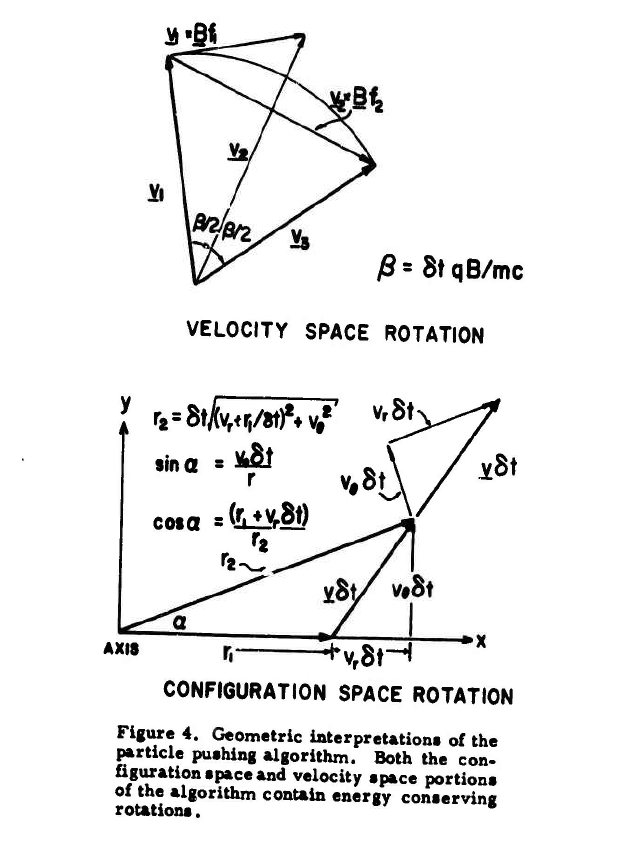
\includegraphics[width=0.6\textwidth]{pics/chap1/boris.png}
  \caption[Illustration of Boris velocity rotation]{Illustration of Boris
    velocity rotation, from \citep{boris_relativistic_1970}}
  \label{fig:boris-velocity-rotation}
\end{figure}


However one can see that an approximation was made in Boris pusher, namely the
average velocity vector between timesteps $i+1/2$ and $i-1/2$ is given by
equation \eqref{eq:boris-average-u}. This is an approximation since
Boris pusher was derived with non-relativistic particle dynamics in mind.
\citet{vay_simulation_2008} pointed out that in the special case where
$\mathbf{E} + \mathbf{u}\times \mathbf{B}/c = 0$ the Boris pusher may introduce a
spurious force on the particles. A better average is simply given by
\begin{equation}
  \label{eq:vay-average-u}
  \mathbf{\bar{u}}^i = \frac{\mathbf{u}^{i-1/2} + \mathbf{u}^{i+1/2}}{2} = \frac{\mathbf{p}^{i-1/2}/\gamma^{i-1/2} + \mathbf{p}^{i+1/2}/\gamma^{i+1/2}}{2m}
\end{equation}
Then the simple Boris scheme is no longer applicable. Vay outlined a new scheme
which is slightly more complicated but more accurate when the Lorentz force of
the particles is almost balanced by the electric force. The procedure is as
follows. One first defines $\mathbf{p}'$ similar to that in Boris pusher
\begin{equation}
  \label{eq:vay-p-prime}
  \mathbf{p}' = \mathbf{p}^{i-1/2} + q\Delta t\left( \mathbf{E}^i + \frac{\mathbf{u}^{i-1/2}}{2c}\times \mathbf{B}^i \right)
\end{equation}
then one can find $\mathbf{p}^{i+1/2}$ and $\gamma^{i+1/2}$ as follows:
\begin{align}
  \label{eq:vay-solution}
  \gamma^{i+1/2} &= \sqrt{\frac{\sigma + \sqrt{\sigma^2 + 4(\tau^2 + p_{*}^2)}}{2}} \\
  \mathbf{p}^{i+1/2} &= s \left[ \mathbf{p}' + (\mathbf{p}'\cdot \mathbf{t})\mathbf{t} + \mathbf{p}'\times \mathbf{t} \right]
\end{align}
where $\bm{\tau} = (q\Delta t/2c)\mathbf{B}^i$, $p_{*}=\mathbf{p}'\cdot\bm{\tau}/c$,
$\sigma = \gamma'^2-\tau^2$, $\gamma' = \sqrt{1 + p'^2/c^2}$, $\mathbf{t} =
\bm{\tau}/\gamma^{i+1/2}$, and $s = 1/(1 + t^2)$.

Since in the simulations of our interest, much of the plasma is both
relativistic and close to force-free, meaning that $\mathbf{E} +
\mathbf{u}\times \mathbf{B}/c$ is close to zero, it is important to use Vay
pusher to avoid spurious forces. Therefore in Aperture we use the Vay pusher
exclusively.

\subsection{Integrating the Maxwell Equations}
\label{sec:fd-maxwell}

In this section we outline how we use the fields $\mathbf{E}^{i}$ and
$\mathbf{B}^{i}$ to compute their values at the next time step. The most
natural way is to use the traditional leapfrog method again
\begin{align}
  \label{eq:maxwell-leapfrog}
  \mathbf{E}^{i+1} &= \mathbf{E}^i + \Delta t (c\nabla\times \mathbf{B}^{i+1/2} - 4\pi \mathbf{j}^{i+1/2}) \\
  \mathbf{B}^{i+1/2} &= \mathbf{B}^{i-1/2} - \Delta t (c\nabla\times \mathbf{E}^i)
\end{align}
This scheme is stable as long as the time step $\Delta t$ satisfies the Courant
condition $\Delta t < \Delta x / c$ where $\Delta x$ is the smallest grid
spacing. However, one difficulty is that in this scheme $\mathbf{E}$ and
$\mathbf{B}$ fields are not defined at the same time step, whereas in our
particle pusher \eqref{eq:leap-frog-ptc-pos} and
\eqref{eq:leap-frog-ptc-momentum} they are implicitly assumed to be sampled at
the same time step.

An improved method we employ is the semi-implicit field solver used by
\citet{haugboelle_photon-plasma:_2012}. We start from the following finite
difference equations:
\begin{align}
  \frac{\mathbf{E}^{i+1} -\mathbf{E}^{i}}{\Delta t} & = c\nabla \times (
  \alpha \mathbf{B}^{i+1} + \beta \mathbf{B}^{i} ) - 4\pi\mathbf{j}^{i+1/2}\\
  \frac{\mathbf{B}^{i+1} -\mathbf{B}^{i}}{\Delta t} & = - c\nabla \times
  ( \alpha \mathbf{E}^{i+1} + \beta \mathbf{E}^{i} )
\end{align}
where $\alpha$ and $\beta$ are numerical parameters that determines
the ``implicitness'' of the scheme, with the constraint $\alpha +
\beta = 1$. If $\alpha \gtrsim 0.5$ then the scheme is unconditionally
stable. Bigger $\alpha$ leads to the damping of grid-scale waves,
which helps smoothing the solution.

To solve these equations, we can plug the first equation into the second one
to eliminate $\mathbf{E}^{i+1}$, explicitly assuming $\nabla\cdot \mathbf{B} =
0$:
\begin{equation}
  \begin{split}
    (1 - \alpha^2\Delta t^2\nabla^2)\mathbf{B}^{i+1} &= \mathbf{B}^i + \alpha\beta \Delta t^2\nabla^2 \mathbf{B}^i \\
    &\phantom{=} -\Delta t\nabla\times \mathbf{E}^i + \alpha\Delta t^2\nabla\times \mathbf{j}^{i + 1/2}
  \end{split}
\end{equation}
Now this is an equation of $\mathbf{B}^{i+1}$ only. We can solve it by inverting
the operator $(1 - \alpha^2\Delta t\nabla^2)$ and apply it to the right hand side
\begin{equation}
  \label{eq:field-relax}
  (1 - \alpha^2\Delta t^2\nabla^2)^{-1} = 1 + \alpha^2\Delta t^2\nabla^2 + (\alpha^2\Delta t^2\nabla^2)^2 + \dots
\end{equation}
Provided $\Delta t$ is small enough, this series converges rapidly. Practically
we found that it is sufficient to terminate the series at around 4 terms, giving
a relative numerical error less than $10^{-8}$. Thus, although the Laplace
operator is a global operation and a global exchange of guard cell values is
required, the field solver is still significantly faster than the particle
pusher, rendering the overhead negligible. Again, see section
\ref{sec:code-aperture} for more detail on domain decomposition and the usage of
guard cells.

One particular note is that if higher order numerical differential operators
were used in current deposition, then the same order of differential operators
should be used here in the field evolution, otherwise the exact charge
conservation will not be imposed. This is because we need the curl of
$\mathbf{B}$ to be divergence-free to numerical precision, which is only true
when the divergence and curl are evaluated to the same order of accuracy with
the same staggering structure (see section \ref{sec:discretization}). This will
be discussed in more detail in appendix \ref{app:finite-diff}.

\subsection{Coordinate Systems and Boundary Conditions}
\label{sec:coord-syst-sing}

Aperture supports the use of orthogonal curvilinear coordinate systems, which
basically means any parametrization of the Euclidean $\mathbb{R}^{3}$ that has a
diagonal metric. The coordinate system can be specified by three scale functions
$h_{i} = \sqrt{g_{ii}}$. Since the metric is diagonal, this contains all the
information of the metric.

The vector operations that we use in solving the Maxwell equations can be
written in terms of these scale functions:
\begin{align}
  \label{eq:vector-derivatives}
  \nabla f &= \frac{1}{h_{i}}\partial_{i}f \\
  \nabla \cdot \mathbf{V} &= \frac{1}{\prod_{k}h_{k}}\partial_i(V_i\prod_{j\neq i}h_{j}) \\
  \nabla \times \mathbf{V} &= \frac{1}{\prod_lh_l}\mathbf{e}_{i}\epsilon_{ijk}h_i\partial_j(h_kV_k)
\end{align}
where Einstein summation convention is assumed and repeated indices are summed
over (except in the product sign). Due to the general form of these equations,
it is straightforward to implement a general framework that works with vector
derivatives, that can take in any scale functions $h_{i}$.

\begin{table}[h]
  \centering
  \begin{tabular}{lccc}
    \hline
    Coordinate System & $h_1$ & $h_2$ & $h_3$ \\ \hline
    Cartesian ($x$, $y$, $z$) & 1 & 1 & 1 \\ \hline
    Cylindrical ($\rho$, $\theta$, $z$) & 1 & $\rho$ & 1 \\ \hline
    Spherical ($r$, $\theta$, $\phi$) & 1 & $r$ & $r\sin\theta$ \\ \hline
    Log spherical ($x$, $\theta$, $\phi$) & $e^x$ & $e^{x}$ & $e^x\sin\theta$ \\ \hline
  \end{tabular}
  \caption{Scale functions for coordinate systems implemented in Aperture}
  \label{tab:scale-functions}
\end{table}

Although the code was designed with flexibility, the main coordinate systems we
support in the actual code are Cartesian, cylindrical, spherical coordinates and
some of their variants. The scale functions of these coordinate systems are
listed in table \ref{tab:scale-functions}. One particular challenge for each
curvilinear coordinate system is the treatment of particle movement, since
technically one needs to solve the geodesic equation, since the orthonormal
coordinate basis is position dependent. However our curvilinear coordinates are
always a parametrization of $\mathbb{R}^{3}$, so instead of trying to solve for
the geodesic equation, we always convert the position and velocity of the
particle to the corresponding Cartesian values before moving it, where we can
simply use the equation \eqref{eq:eom-position} to update particle position.


\begin{figure}[h]
  \centering
  \begin{tikzpicture}
    \begin{scope}[xshift=-0.5cm]
      \coordinate (A) at (0, 0);
      \draw (A) ++(75:2.0) -- ++(75:4.0);
      \draw (A) ++(45:2.0) -- ++(45:4.0);
      \draw (A) ++(15:2.0) -- ++(15:4.0);
      \draw (A) ++(85:3.0) arc (85:7:3.0);
      \draw (A) ++(85:5.0) arc (85:7:5.0);
      \draw[thick, ->, dashed] (A) ++ (35:3.4) node[above] {$\mathbf{x}_\mathrm{sph}$} -- ++(1.2,-0.4) node[right] {$\mathbf{x}_\mathrm{sph}'$};
    \end{scope}
    \node[single arrow,draw,fill=black!10,minimum width=2cm,minimum height=0.5cm,anchor=west,single arrow head extend=0.3cm] at (5.7,4.5) {$\mathbf{x}_\mathrm{sph} \Rightarrow \mathbf{x}_{c}$};
    \node[single arrow,draw,fill=black!10,minimum width=2cm,minimum height=0.5cm,anchor=west,single arrow head extend=0.3cm,shape border rotate=180] at (5.7,1.5) {$\mathbf{x}'_{c} \Rightarrow \mathbf{x}'_\mathrm{sph}$};
    \begin{scope}[xshift=9.0cm]
      \draw (0,1.0) -- (6.0,1.0);
      \draw (0,3.0) -- (6.0,3.0);
      \draw (0,5.0) -- (6.0,5.0);
      \draw (1.0,0.0) -- (1.0,6.0);
      \draw (3.0,0.0) -- (3.0,6.0);
      \draw (5.0,0.0) -- (5.0,6.0);
      \draw[thick, ->] (0,0) ++ (35:3.4) node[left] {$\mathbf{x}_{c}$} -- ++(1.2,-0.4) node[right] {$\mathbf{x}_{c}'$};
    \end{scope}
    % \draw (A) -- ++(75:4.0);
  \end{tikzpicture}
  \caption[Particle movement in curvilinear coordinates.]{Particle movement in
    curvilinear coordinates. The particle position and momentum are transformed
    into the corresponding Cartesian values, moved in a straight line, and then
    transformed back to curvilinear coordinates.}
  \label{fig:particle-move}
\end{figure}

An additional challenge in implementation of the coordinate systems
has to do with how boundary singularities are treated, which varies for
different coordinate systems. We will outline the treatment for the axis
boundary in the spherical coordinates here since it is the one implemented
first, and most relevant for the physics applications detailed in the later part
of the thesis.

\subsubsection{Coordinate boundary condition}
\label{sec:coord-bc}

For 2D spherical coordinates, axisymmetry means $\partial_{\phi} = 0$ in all
Maxwell equations. By symmetry, we automatically have on the axis
\begin{equation}
  E_{\theta} = E_{\phi} = B_{\theta} = B_{\phi} = 0
\end{equation}
simply because there is no preferred direction of these field components.
Furthermore, since we have $B_{\phi} = E_{\phi} = 0$ at the boundary for all
times, their time derivatives should vanish, which makes the following
conditions on the axis:
\begin{equation}
  \partial_r(rB_{\theta}) - \partial_{\theta}B_r = 0,\quad \partial_r(rE_{\theta}) - \partial_{\theta}E_{r} = 0
\end{equation}
Since $B_{\theta} = E_{\theta} = 0$ on the axis, so are their $r$
derivatives, therefore we have instead
\begin{equation}
  \partial_{\theta}B_r = \partial_{\theta}E_r = 0
\end{equation}
which is akin to a ``symmetric'' boundary condition for both $E_r$ and $B_r$.

For the actual boundary conditions we have to impose on the fields, we need to
refer to the staggered grid configuration (figure \ref{fig:Yee}). Our simulation
domain boundary coincides with the spherical axis $\theta = 0$, $\pi$; then 4
components will be defined exactly on the boundary: $B_{\phi}$, $E_{\theta}$,
$E_r$, and $j_{\theta}$. From the discussion above, we immediately have
$B_{\phi} = E_{\theta} = 0$. We impose this condition simply as a Dirichlet
boundary condition every timestep, by setting these field components to zero for
all the cells on the axis.

Similarly, $j_{\theta}$ should also be zero. This is handled by slightly
modifying the current deposition step: every particle that moves in the cells
adjacent to the axis boundary is assigned a ghost particle that is its mirror
image across the axis. The resulting $\Delta \rho$ is taken to be the average
from the movement of both particles. This symmetric construction automatically
guarantees that $j_{\theta} = 0$ on the boundary. This also serves as a suitable
starting point for the current prefix sum for $j_{\theta}$ since we know that it
always starts from 0 at $\theta = 0$.

Finally for $E_{r}$, its update equation is:
\begin{equation}
  \label{eq:Er-update}
  \partial_tE_r = \frac{1}{r\sin\theta}\partial_{\theta}\sin\theta B_{\phi}
\end{equation}
The difficulty here is that $\sin\theta \to 0$ as $\theta\to 0$ or
$\theta\to\pi$ at the axis. Our way to solve this issue is to take the limit:
\begin{equation}
  \label{eq:biot-savart}
  \lim_{\theta\to 0}\partial_tE_r = \lim_{\theta \to 0}\frac{\sin\theta\partial_{\theta} B_{\phi} + \cos\theta B_{\phi}}{r\sin\theta} = \frac{1}{r}\partial_{\theta}B_{\phi} + \lim_{\theta\to 0}\frac{\partial_{\theta}(\cos\theta B_{\phi})}{\partial_{\theta}(r\sin\theta)} = \frac{2}{r}\partial_{\theta}B_{\phi}
\end{equation}
The only remaining complication here is that to evaluate
$\partial_{\theta}B_{\phi}$ we can't use the information across the axis and
need to rely on the cells within the physical domain. Therefore one cannot use
the symmetric finite difference operator (equation
\eqref{eq:finite-diff-2nd-order}). One can however use the information that
$B_{\phi}$ is zero on the boundary. To get the same 2nd order accuracy in
$\Delta \theta$, we can use:
\begin{equation}
  \label{eq:one-sided-2nd-order}
  \partial_\theta B_{\phi} = 2B_{\phi}(\Delta\theta) - \frac{1}{2}B_{\phi}(2\Delta \theta) + O(\Delta \theta^{3})
\end{equation}
We will discuss this in more detail and the extension to higher order in
appendix \ref{app:finite-diff}.

\subsubsection{Stellar boundary condition}
\label{sec:stellar-bc}

In magnetospheric simulations, the inner boundary of the box is always the
neutron star itself. The stellar boundary is treated as a perfect conductor:
$\mathbf{E} = -\mathbf{v}_\mathrm{rot}\times \mathbf{B}/c$ and $\mathbf{B} =
\mathbf{B}_\mathrm{dipole}$ below the surface. $\mathbf{v}_\mathrm{rot} =
\mathbf{r}\times \bOm$ is the rotation velocity of the star; it determines
$\mathbf{E}$ at the surface and this is how the simulation knows about the
rotation of the star. Typically at the beginning of the simulation
$\mathbf{v}_\mathrm{rot}$ is taken to be identically zero, and the star is spun
up smoothly over a relatively short time frame. For magnetar simulations, it is
the differential rotation of the star that we impose, which is done through an
latitude dependent $\mathbf{v}_\mathrm{rot}(\theta)$, and the rotation of the star
is ignored (see chapter \ref{chap:magnetar}).

Particles are injected into the simulation domain below the surface in pairs of
electrons and ions. In order to not introduce artificial charges into the
simulation, they are injected at exactly the same location with only a small
random thermal velocity. Particles entering the star are erased once they
penetrate deep enough such that all cells they contribute the current to are
below the surface. This is again to avoid violating the Gauss's law inside the
simulation domain, since erasing charges in general introduce errors to the
Gauss's law.

For magnetospheric simulations we also implemented gravity for all particles to
control the injection layer. Injected particles have a thermal momentum
distribution with mean momentum $\bar{p}_{0}$, and gravity is implemented with a
force profile of $\mathbf{g} = -\hat{\mathbf{r}}mg_0/r^{2}$. The parameter $g_0$
controls the strength of gravity, as well as the thickness of the atmospheric
layer, $h \sim v_0^{2}/2g_0$. In the beginning of the simulation, the star
starts at rest to allow the formation of a dense atmosphere. The use of this
atmospheric layer ensures that there is always an abundant supply of particles
from the surface, and decouples it from the detail of actual particle injection
at each timestep.

\subsubsection{Free escape boundary condition}
\label{sec:escape-bc}

The outer boundary uses a free escape condition. To achieve this we place a
damping layer at the outer boundary as described by \citet{umeda_improved_2001}.
The damping layer is placed near $r_\mathrm{max}$ in which the field values at
every time step is multiplied by a masking function that depends on the radial
position $r$:
\begin{align}
  % \label{eq:damping}
  \mathbf{E}^{n+1} &= f_M(r) \left[ \mathbf{E}^i + c\Delta t\nabla \times \left( \alpha
                     \mathbf{B}^{i+1} + \beta \mathbf{B}^i \right) - 4\pi
                     \Delta t\mathbf{j}^{i+1/2} \right] \\
  \mathbf{B}^{n+1} &= f_{M}(r) \left[ \mathbf{B}^i - c\Delta t\nabla \times \left(
                     \alpha \mathbf{E}^{i+1} + \beta \mathbf{E}^i \right) \right]
\end{align}
and we adopt the masking function used in \citep{umeda_improved_2001}:
\begin{equation}
  \label{eq:masking-function}
  f_M(r) =
  \begin{cases}
    \displaystyle 1, & \mathrm{for\ }r < r_D \\
    \displaystyle 1 - \eta\left( \frac{r - r_D}{r_\mathrm{max} - r_D} \right)^2, & \mathrm{for\ }r \geq r_{D}
  \end{cases}
\end{equation}
where $r_{D}$ is where the damping layer begins, and $\eta$ is a numerical
coefficient that controls the effectiveness of the damping. In the simulations,
the damping layer is usually chosen to be 10 to 15 cells, and $\eta$ is chosen
to be small such that the characteristic skin depth of waves into the medium is
similar to the damping layer thickness. In other words, the coefficient is
chosen that the waves are damped slowly enough to not generate much reflection.
In practice, the wave damping is very efficient, and wave reflection is very
weak for all production runs.

It is very common for PIC codes to implement a perfectly-matched layer (PML) as
an absorbing boundary condition \citep{berenger_perfectly_1994}. We have also
implemented it and compared it with the effectiveness of the simple damping
layer. We found that the result is almost identical, but since the damping layer
is more efficient in terms of computation and memory, we decided to keep this
implementation.

Particles streaming into the damping layer decouples from the field and are
allowed to freely escape from the box. When they enter the guard cells located at
the outer boundary, they are erased.



% TODO: Finish boundary conditions

% The more important boundary condition is not on the fields, but on the
% differential operators. Naively one might want to just apply the most
% general differential operator on all points, and then correct for the
% fields afterwards, but that approach is not ideal when higher order
% differential operators are involved, nor is it appropriate when one
% wants to chain several differential operators together to evaluate,
% say, $\nabla\times(\nabla\times \mathbf{B})$.

% Therefore let us reformulate the problem into finding the appropriate
% boundary condition for $\nabla\times \mathbf{E}$ and $\nabla\times
% \mathbf{B}$ at the axis $\theta = 0$, $\pi$. The differential operator
% looks like the following:
% \begin{equation}
%   \begin{split}
%     \nabla\times \mathbf{E} &= \hat{\mathbf{r}}\frac{1}{r\sin\theta}\partial_{\theta}^-\sin\theta E_{\phi} \\
%     &- \hat{\bm{\theta}}\frac{1}{r}\partial_r^-rE_{\phi} \\
%     &+ \hat{\bm{\phi}}\left( \frac{1}{r}\partial_r^-rE_\theta - \frac{1}{r}\partial_{\theta}^-E_r \right)
%   \end{split}
% \end{equation}
% And similar for $\mathbf{B}$. Note that all differential operators are
% $\partial^-$ in the case of $\nabla\times \mathbf{E}$, and
% $\partial^+$ in the case of $\nabla\times \mathbf{B}$. Near the axis,
% the problematic terms are the $\partial_{\theta}$ derivatives. That
% means the $\partial_{\theta}\sin\theta E_{\phi}$ term and the
% $\partial_{\theta}E_r$ term.

% For the later, we have the powerful condition that right on the axis
% $\partial_{\theta}E_r = 0$. In fact, we have $(\nabla\times
% \mathbf{E})_{\phi} = 0$ at the axis boundary. For $\nabla\times
% \mathbf{E}$, it is directly evaluated on the boundary, therefore we
% impose the above condition directly on the boundary cell. For the cell
% in the box directly next to the boundary, we use the modified
% one-sided 4th order scheme:
% \begin{equation}
%   \label{eq:1-sided-4th-order}
%   \partial_{\theta}^-E_{i,j}^r = \frac{1}{\Delta r}\left[-\frac{11}{24} E_{i,j}^{r} + \frac{17}{24}E_{i+1,j}^{r} + \frac{3}{8}E^{r}_{i+2,j} - \frac{5}{24}E^{r}_{i+3,j} + \frac{1}{24}E^r_{i+4,j} )\right]
% \end{equation}
% Since $E_{\phi}$ and $E_r$ are similarly staggered in the $\theta$
% direction, same formula applies. Points further into the box do not
% feel the presence of the boundary.

% For the former term it is a bit tricky, since the coefficient
% $1/r\sin\theta$ vanishes at the axis. A limit analysis reveals that
% \begin{equation}
%   \lim_{\theta\to 0}\frac{1}{r\sin\theta}\partial_{\theta}\sin\theta E_{\phi} = \frac{2\partial_{\theta}E_{\phi}}{r}
% \end{equation}
% And since $(\nabla\times \mathbf{E})_r$ is directly evaluated on the
% axis boundary, we need to use the above formula to compute its
% value. When computing the derivative $\partial_{\theta}E_r$, we can
% use an even more extreme version of the 4th-order one-sided
% derivative:
%     % return (-f1 * 31.0 / 8.0 + f2 * 229.0 / 24.0 - f3 * 75.0 / 8.0 + f4 * 37.0 / 8.0 - f5 * 11.0 / 12.0) / delta;
% \begin{equation}
%   \partial_{\theta}^-E_{i,j}^\phi = \frac{1}{\Delta r}\left[-\frac{31}{8} E_{i+1,j}^{\phi} + \frac{229}{24}E_{i+2,j}^{\phi} - \frac{75}{8}E^{\phi}_{i+3,j} + \frac{37}{8}E^{\phi}_{i+4,j} - \frac{11}{12}E^\phi_{i+5,j} )\right]
% \end{equation}
% However, there is one piece of information we can use, which is the
% fact that $E_{\phi} = 0$ on the boundary. If taken this condition into
% account, then we can reduce the above equation into the modified
% one-sided derivative:
% \begin{equation}
%   \partial_{\theta}^-E_{i,j}^\phi = \frac{1}{\Delta r}\left[\frac{35}{8} E_{i+1,j}^{\phi} - \frac{35}{24}E_{i+2,j}^{\phi} + \frac{21}{40}E^{\phi}_{i+3,j} - \frac{5}{56}E^{\phi}_{i+4,j} )\right]
% \end{equation}

% For $\nabla\times \mathbf{B}$ the analysis is similar. However, due to
% the difference in staggering scheme, different components are
% evaluated at the boundary. Therefore different boundary considerations
% apply. For the $\partial_{\theta}B_r$ term, since it is not evaluated
% directly on the boundary, we need only use the one-sided derivative
% \eqref{eq:1-sided-4th-order} for the point closest to the boundary.

% For the $\partial_r(\sin\theta B_{\phi})/r\sin\theta$ term, again it
% is not evaluated directly on the boundary, therefore we only need to
% use \eqref{eq:1-sided-4th-order} on the point closest to the boundary,
% similar to the above term.

% The analysis up to this point completely fixes $\nabla\times
% \mathbf{E}$ and $\nabla\times \mathbf{B}$ at the axis boundary. Even
% if our $\theta$ boundary is not taken to be exactly at $\theta = 0$,
% $\pi$, the above conditions should still approximately hold. Plus,
% since the evaluation of the curl does not need anything from the ghost
% cells, we can evaluate $\nabla\times(\nabla\times \mathbf{B})$ with no
% problem.

% If we want to implement the semi-implicit scheme, then we need to fix
% the boundary condition for the differential operator $\nabla\cdot
% \mathbf{B}$ at the axis as well. We have
% \begin{equation}
%   \begin{split}
%         \nabla\cdot \mathbf{B} &= \frac{1}{r^2}\partial_r^-(r^2B_r) + \frac{1}{r\sin\theta}\partial_{\theta}^-(\sin\theta B_{\theta}) \\
%         &= \frac{1}{r^3\sin\theta}\left[ \partial_x^-(r^2\sin\theta B_r) + \partial_{\theta}^-(r^2\sin\theta B_{\theta}) \right]
%     \end{split}
% \end{equation}
% The second line is written out explicitly in log-spherical
% coordinates. Both terms present a challenge since $\sin\theta$ is zero
% on the axis. The second term reduces to
% $2\partial_{\theta}B_{\theta}/r$ similar to what happens before, and
% can be dealt with using the modified one-sided derivative
% \eqref{eq:14}. This is actually the property of the
% $\partial_{\theta}^-$ operator. The first term need to be evaluated
% with $\sin\theta$ moved out from the derivative, and this needs to be
% done in the code by hand as a special case.

% Lastly we have the gradient operator. We actually have two different
% versions depending on whether $f$ is evaluated at the center of the
% cell or at the corner of the cell. If we call the former $f^-$ and the
% latter $f^+$, then
% \begin{equation}
%   \nabla f^- = \hat{\mathbf{r}}\partial_r^-f + \hat{\bm{\theta}}\frac{1}{r}\partial_{\theta}^-f
% \end{equation}
% and similar for $f^+$. Obviously $\nabla\cdot \mathbf{B}$ belongs to $f^+$.
% % and the two components have the same stagger structure as $\mathbf{B}$
% % if $f = \nabla\cdot \mathbf{B}$.
% % The problem near the axis arises in the second term in the $\theta$
% % derivative.
% Since the derivative involved is $\partial^+$ and therefore not
% evaluated on the axis, simply using \eqref{eq:1-sided-4th-order} near
% the axis will fix the problem.


\subsection{Radiative Transfer}
\label{sec:radiative-transfer}

A significant feature of Aperture compared to traditional PIC codes is the
inclusion of various radiative transfer mechanisms that are important in
high-energy astrophysics. In this section we list the supported physical
processes and outline how we model them in the code.

\subsubsection{Production of high energy photons}
\label{sec:instant-pair}

In the magnetosphere of neutron stars, energetic electrons or positrons can
induce vacuum breakdown and create $e^{\pm}$ pairs. This is usually a 2-step
process. First, a high energy photon ($E_\mathrm{ph} > 2m_{e}c^2$) is emitted
from the energetic particle, and the photon will then convert into a pair of
$e^{\pm}$. In pulsar magnetospheres, the first process is typically from
curvature radiation from electrons accelerated to Lorentz factors $\gamma
\gtrsim 10^{6}$ (see discussion in section \ref{sec:gap-models}). Another
channel for producing highly energetic photons capable of converting into
$e^{\pm}$ pairs is from resonant upscattering of background X-ray photons. The
electron absorbs photons that have the energy to excite it from the lowest
Landau level to the first excited level, and subsequently drop down to the
lowest level, re-emitting the photon. The photon energy in the lab frame is
boosted by a factor of $\gamma^2$ during this process, similar to ordinary
inverse Compton scattering.

% However in magnetars where the magnetic field is much stronger, the energetic
% photons mainly come from resonantly up scattered X-ray photons from either the
% thermal emission from the surface of the star, or from synchrotron emission of
% the plasma in the magnetic field.

{\it Aperture} models both channels of high-energy photon emission with a threshold
condition and an emission rate. For curvature radiation, we compute the local
radius of curvature of the particle trajectory using
\begin{equation}
  \label{eq:curvature-radius}
  R_{c} = \frac{|\mathbf{p}|^3\Delta t}{\gamma \left| \mathbf{p} \times \Delta \mathbf{p} \right|}
\end{equation}
and then we set the threshold for emitting a curvature photon that is capable of
converting to a pair to be
\begin{equation}
  \label{eq:curvature-threshold}
  \gamma_\mathrm{th} = K(R_{c}/R_{*})^{1/3}
\end{equation}
where $K$ is a numerical parameter that we can tune to fit the parameter space
for the simulation. In real pulsars this coefficient can be $K\gtrsim 10^{6}$.
The photon energy emitted is artificially set to be a certain multiple of
$m_{e}c^2$ which is another numerical parameter that affects the final pair
multiplicity.

For resonant scattering we can set the threshold condition to be exactly the
resonance condition for the local $B$ field:
\begin{equation}
  \label{eq:resonant-threshold}
  \gamma_\mathrm{th} = \gamma_0\frac{B}{B_Q}
\end{equation}
where $B_Q$ is the critical field for QED effects, $B_Q = m^2c^3/e\hbar =
4.4\times 10^{13}\,G$. It was found that in the realistic magnetar outflow the
threshold scales as $\gamma_\mathrm{th} \sim 100 B/B_{Q}$
\citep{beloborodov_mechanism_2013}, but this coefficient can be tuned for the
particular range of parameters used in a simulation.

The energy of the emitted photon is set by the local magnetic field as well. The
energy of the emitted photon for a given resonant scattering event is given by
\citep{beloborodov_corona_2007}
\begin{equation}
  \label{eq:resonant-emit-Eph}
  E_\mathrm{ph}(\theta_\mathrm{em}) = \frac{E_B}{\sin^2\theta_\mathrm{em}}\left[ 1 - \left(\cos^2\theta_\mathrm{em} + \frac{m_{e}^2c^4}{E_B^2}\sin^{2}\theta_\mathrm{em}} \right)^{1/2} \right]
\end{equation}
where $\theta_\mathrm{em}$ is the emission angle of the de-excitation photon
with respect to the $B$ field in the frame where the parallel momentum of the
electron/positron vanishes. $E_{B}$ is the energy of the first Landau level:
\begin{equation}
  \label{eq:first-landau}
  E_{B} = \left( \frac{2B}{B_Q} + 1 \right)^{1/2}m_{e}c^2
\end{equation}
In the actual code, we use the angle-averaged version of equation
\eqref{eq:resonant-emit-Eph} \citep{beloborodov_mechanism_2013}
\begin{equation}
  \label{eq:average-Eph}
  E_\mathrm{ph} = \gamma m_{e}c^{2}\left( 1 - \frac{1}{1 + 2B/B_{Q}} \right)
\end{equation}
and in the very narrow parameter range when this energy is greater than $(\gamma
- 1)m_{e}c^2$ we cap the emitted photon energy at $(\gamma - 1)m_{e}c^2$.

\subsubsection{Conversion of high energy photon into pairs}
\label{sec:pair-create}

% Aperture tracks high energy photons created through either channel described
% above. There are two modes for converting into an $e^{\pm}$ pair. When the
% ambient magnetic field is strong ($\gtrsim 10^{12}\,\mathrm{G}$), the photon can
% interact with the magnetic field and convert to an $e^{\pm}$ pair immediately.
% The condition for this magnetic conversion is that the angle $\theta$ between
% the propagation direction of the photon and the direction of the magnetic field
% should be large enough:
% \begin{equation}
%   \label{eq:magnetic-conversion-condition}
%   E_\mathrm{ph} > \frac{m_{e}c^2}{\sin\theta}
% \end{equation}

It is impossible for a photon to convert into $e^{\pm}$ spontaneously due to
inability to conserve both energy and momentum. There are two main channels for
energetic photons to convert into an $e^{\pm}$ pair: through interaction with the
local $B$ field, or through collision of two energetic photons.

Magnetic conversion has strict requirement on the strength of $B$ field. The
rate decreases exponentially with respect to $B/B_{Q}$
\citep{erber_high-energy_1966}. In addition, the photon propagating at an angle
$\theta$ with respect to the $B$ field has to satisfy the threshold condition
\begin{equation}
  \label{eq:magnetic-conversion-condition}
  E_\mathrm{ph} > \frac{m_{e}c^2}{\sin\theta}
\end{equation}
We model the exponential cross section for the magnetic conversion as a sharp
cut-off $B_\mathrm{th}$ below which magnetic conversion simply turns off. When
local $B$ field is larger than $B_\mathrm{th}$ then the energy of the photon is
compared to the threshold energy \eqref{eq:magnetic-conversion-condition} and
pair creation is triggered when the condition is satisfied.

In the outer regions of the magnetosphere $B$ quickly falls far below $B_{Q}$
and magnetic conversion is prohibited. The only channel becomes
$\gamma$-$\gamma$ collision. It is extremely difficult to compute the background
target field for the high energy photons to collide with, since it is produced
by both thermal emission from the star and synchrotron radiation from the
particles in the magnetosphere. Instead of calculating the target field, we
assume a random photon free-path:
\begin{equation}
  \label{eq:photon-free-path}
  \ell_\mathrm{ph} \sim \mathcal{N}(aR_{*}, (bR_{*})^2)
\end{equation}
where $\mathcal{N}(\mu, \sigma^2)$ denotes a normal distribution with mean $\mu$
and variance $\sigma^2$, and $a$ and $b$ are parameters we choose (see chapter
\ref{chap:pulsar}). The normal distribution is truncated at $\ell_\mathrm{ph} =
0$ and any negative value is discarded. Every photon is produced with a
free-path drawn from distribution \ref{eq:photon-free-path}, and if it is not
converted magnetically or escapes the domain, then it is converted to a pair of
$e^{\pm}$ at the end of its free path. The energy of the photon is evenly shared
by the resulting electron and positron, while the momenta of these particles are
along the same direction as the original photon.

Although unphysical, this approximation captures the qualitative behavior of
a pair cascade in the pulsar magnetosphere, producing the required amount of
plasma in the correct regions. A more sophisticated modeling of the pair
creation process will definitely improve the calculation of local pair density
in the magnetosphere, but the overall structure of the system will remain
unchanged, since it is close to the force-free limit already.

\subsubsection{Synchrotron and general radiative loss}
\label{sec:synchrotron-loss}

When energetic particles gyrate in a magnetic field they emit synchrotron
radiation. Even when the synchrotron (or curvature) photons are not energetic
enough to produce pairs, their emission can result in significant energy loss of
particles, which may affect the global dynamics of plasma and fields.
% in the X-ray to soft gamma-ray band. Since the energy of these
% synchrotron photons is in general much less than $m_{e}c^{2}$, we do not track
% them explicitly. However, charged particles do lose energy to synchrotron
% radiation and it may affect the global dynamics.
In Aperture we implemented a general radiative damping force to account for the
synchrotron and curvature radiation loss that is not explicitly tracked by
photon production. The radiation power by a moving particle in an
electromagnetic field is \citep[see e.g.][]{longair_high_2011}:
\begin{equation}
  \label{eq:rad-power}
  \mathcal{P}_\mathrm{rad} = \frac{2e^2}{3c^3}\gamma_{e}^{4}(a_{\perp}^2+\gamma_{e}^2a_{\parallel}^2)
\end{equation}
where $\perp$ and $\parallel$ are with respect to the direction of motion of the
particle. The radiative damping force acting on relativistic particles is given by:
\begin{equation}
  \label{eq:rad-force}
  \mathbf{F}_\mathrm{rad} = -\frac{\mathcal{P}_\mathrm{rad}}{c^2}\mathbf{p}
\end{equation}

% TODO: Put up the full force formula

\subsubsection{Radiative drag due to resonant scattering}
\label{sec:resonant-scattering}

In the magnetospheres of magntars, resonant scattering plays a crucial role in
the particle dynamics. The relativistic outflow of $e^{\pm}$ pairs is bathed in
a background of X-ray photons that come from the thermal emission from the star;
as the particles flow along the field lines, they sample different part of the
photon spectrum.

We simplify the problem by ignoring the contribution to the X-ray spectrum from
the flow itself, and only consider thermal photons from the star. This way one
can compute analytically the effect of resonant scattering on the particle flow.
The central blackbody radiation on average applies a force on the particles
\citep{beloborodov_electron-positron_2012}:
\begin{equation}
  \label{eq:resonant-drag}
  \mathcal{F}(\beta) = \frac{\alpha^2R_{*}^2}{4r^2}\frac{m_{e}c^2}{r_{e}}\Theta^3\gamma g(y)(\beta_{*}-\beta)
\end{equation}
where $\beta_{*} = \mu = B_r/B$, $\Theta = kT/m_{e}c^2$ is the surface
temperature in units of electron rest mass, and
\begin{equation}
  \label{eq:y-and-gy}
  g(y) = \frac{y^3}{e^y - 1},\quad y = \frac{\hbar\omega_\mathrm{res}}{kT} = \frac{B/B_Q}{\gamma(1 - \beta\mu)\Theta}
\end{equation}

The effect of the force \eqref{eq:resonant-drag} is pushing the flow velocity
towards the ``radiatively locked flow'' velocity $\beta_{*}$. Numerically we
implement the force with two parameters:
\begin{equation}
  \label{eq:resonant-drag-numerical}
  \frac{d\mathbf{p}}{dt} = \mathcal{F}(\mathbf{p}) = \mathcal{D}\frac{g(y)}{(r/R_{*})^2}(\gamma\mu - p)
\end{equation}
and the direction of this force is along the $B$ field. The two numerical
parameters are $\mathcal{D}$ and $\Theta$. The former determines the overall
strength of the drag, and the second determines which part of the thermal
spectrum interacts with the particles. Depending on these two parameters, a
certain part of the field line bundle will have particles stopping at the
equator since $\beta_{*} = \mu = 0$ at the equator. In the inner magnetosphere
where $B$ field is too strong ($B \gtrsim B_{Q}$) only very high energy
particles resonantly scatter thermal photons, and the drag is not enough to stop
particles near the equator. The scenario described in chapter
\ref{chap:magnetar} applies to this region. For very extended field lines the
drag is too weak since it scales with $r^{-2}$, and particles are not stopped at
the equator either.

% TODO: expand a bit this section

% \subsection{Organization of the Code}
% \label{sec:code-organization}

\subsection{Units}
\label{sec:pic-units}

% A computer simulation is ignorant of the physical units of the dynamic
% variables, therefore one should choose a unit for all physical quantities, such
% that in the code all quantities are pure numbers.
In a computer simulation it is convenient to deal with dimensionless quantities,
expressed in some units of choice. It is to our benefit to choose a unit system
that is most natural to the problem and in which the dynamic equations take the
simplest dimensionless form. Our choice of units is described in this section.
This process also highlights the relevant scales of the problem.

The primary goal of the code is to simulate an isolated neutron star, therefore
the natural length scale is the stellar radius $R_{*}$, and there is no other length
scale {\it a priori}. Naturally, the time scale of the problem would be the
light-crossing time of the star. Therefore we define the dimensionless length
and time using the following equations (in all the following equations, a tilde
on the symbol means the dimensionless version):
\begin{equation}
  r = \tilde{r}R_{*},\quad t = \tilde{t}\frac{R_{*}}{c},\quad \omega = \tilde{\omega}\frac{c}{R_{*}}
\end{equation}
The radius $\tilde{r} = 1$ shows up mainly as the lower boundary of most of our
simulations.

Once we add rotation of the star and a magnetic field, two important frequencies
show up in this problem that can then be written in dimensionless units:
\begin{equation}
  \tilde{\Omega} = \frac{\Omega R_{*}}{c},\qquad \tilde{\omega}_B = \frac{\omega_BR_{*}}{c} = \frac{e B_0R_{*}}{mc^2}
\end{equation}
where $m$ is the electron rest mass, $\Omega$ is the rotation angular frequency,
equal to $2\pi / P$ where $P$ is the period of rotation, and $B_0$ is the
surface magnetic field at the pole. Given a pulsar with certain radius, these
two are the dimensionless parameters that will govern the simulation, and hence
the physical behavior of the system.

Next, we need to define a unit for charge density. This can be done by relating
the plasma frequency, a third frequency in the problem, with the local
corotation charge density $\rho_\mathrm{GJ} = -\bOm\cdot \mathbf{B}/2\pi c$. We
define the reference plasma frequency at every point as
\begin{equation}
  \omega_p^2 = \frac{4\pi \rho_\mathrm{GJ}e}{m}
\end{equation}
then we can define a version of dimensionless Goldreich-Julian density, or any charge density
\begin{equation}
  \rho_\mathrm{GJ} = \frac{m \tilde{\omega}_p^2 c^2}{4\pi e R_{*}^2} = \tilde{\rho}_\mathrm{GJ} \frac{mc^2}{4\pi eR_{*}^2}
\end{equation}
Note that the real plasma frequency will depend on the actual plasma number
density at the point of interest and will in general be different from what we
call $\omega_p$ above. However, it is still useful to determine such a
characteristic plasma frequency for reference. What the above equation says is
that, by choosing these units we make $\tilde{\rho} = \tilde{\omega}_p^2$.
Especially, there is a simple relationship between the three characteristic
frequencies in the problem, if we define $\rho_{GJ} = \Omega B_0 / 2\pi c$:
\begin{equation}
  \frac{m \omega_p^2}{4\pi e} = \frac{\Omega B_0}{2\pi c} \quad \Longrightarrow \quad \tilde{\omega}_p^2 = 2\tilde{\Omega} \tilde{\omega}_B
\end{equation}
Therefore, specifying the numerical values of $\tilde{\Omega}$ and
$\tilde{\omega}_B$ automatically determines the characteristic plasma frequency
in the problem.

With the above choices, we can work out the dimensionless electric and magnetic
fields. Gauss's law gives
\begin{equation}
  \nabla\cdot \mathbf{E} = 4\pi \rho \quad \Longrightarrow \quad \frac{\Delta E}{\Delta \tilde{r} R_{*}} = \tilde{\rho} \frac{m c^2}{e R_{*}^2} \quad \Longrightarrow \quad E = \tilde{E}\frac{m c^2}{e R_{*}}
\end{equation}
and similarly
\begin{equation}
    B = \tilde{B}\frac{m c^2}{e R_{*}}
\end{equation}
Note that this means that $B$ and $\omega_B$ have the same dimensionless form,
therefore $\tilde{B}_0 = \tilde{\omega}_B$.

In these units, Maxwell equations look as follows:
\begin{equation}
  \partial_t \tilde{\mathbf{E}} = \tilde{\nabla}\times \tilde{\mathbf{B}} - \tilde{\mathbf{j}},\quad \partial_t \tilde{\mathbf{B}} = - \tilde{\nabla}\times \tilde{\mathbf{E}}
\end{equation}
and the particle equations of motion become
\begin{equation}
  \frac{d \tilde{\mathbf{p}}}{d \tilde{t}} = \tilde{\mathbf{E}},\quad \frac{d \tilde{\mathbf{r}}}{d \tilde{t}} = \tilde{\mathbf{u}} = \frac{\tilde{p}}{\sqrt{1 + \tilde{p}^2}} \tilde{\mathbf{p}}
\end{equation}
Note that all numerical coefficients disappear.

Up to now, the only numerical parameters we have introduced are $\tilde{\Omega}$
and $\tilde{\omega}_B$, and they completely specify the problem. For simulation
purposes, one needs to rescale both of these parameters to bring the size of the
system into computable regime. However, one more numerical parameter is required
for interpolating between the particle charge and the charge density on the
grid, namely the charge of an individual macro particle. Since in PIC there is
no way to simulate realistic plasma of order $10^{20+}$ particles, one needs to
use one single macro particle to represent a collection of physical particles. A
macro particle has the same charge-to-mass ratio as a physical particle. The way
we choose the charge per particle is to normalize it so that our characteristic
charge density $\rho_\mathrm{GJ}$ would correspond to a certain manageable
number of particles $N_p$ per grid cell.

The way we compute charge density is to iterate over all particles and deposit
onto a single cell:
\begin{equation}
    \rho_c = \frac{\sum e S(\mathbf{r}_p, \mathbf{r}_c)}{\Delta V}
\end{equation}
where $e$ is the charge per macro particle, $S$ is a shape factor depending on
particle position $\mathbf{r}_p$ and grid point position $\mathbf{r}_c$, and
$\Delta V$ is the cell volume. In 2.5D simulations, $\Delta V$ involves the
arbitrary size of the third dimension which is the symmetric direction, so we
usually take the size in that direction to be unity. Assuming every particle has
the same charge $e$, and there are $N_p$ particles in the cell, up to a form
factor, we have
\begin{equation}
    \rho = \frac{e N_p}{\Delta V} = \frac{e N_p}{\Delta \tilde{V} R_{*}^{3}} = \tilde{\rho}\frac{mc^2}{4\pi eR_{*}^2}, \quad \tilde{\rho} = \frac{\tilde{e}N_p}{\Delta \tilde{V}}
\end{equation}
so we can identify the dimensionless charge per particle
\begin{equation}
    \tilde{e} = e \frac{4\pi e}{mc^2R_{*}}
\end{equation}
Note that $e$ appears twice on the right hand side. This is because we treat
$e/m$ as a physical constant, therefore $4\pi e / mc^2R_{*}$ is a physical
constant which is fixed as soon as we choose the physical size of the star. We would
like to choose $\tilde{e}$ so that $N_p$ particles per cell corresponds to the
characteristic charge density $\rho_\mathrm{GJ}$:
\begin{equation}
    \tilde{\rho} \sim \frac{\tilde{e} N_p}{\Delta \tilde{V}} \sim \tilde{\rho}_\mathrm{GJ} \quad \Longrightarrow \quad \tilde{e} = \frac{2\tilde{\Omega} \tilde{B}\Delta \tilde{V}}{N_p}
\end{equation}

One technical aspect about the numerical value $\tilde{e}$ in the code is that,
every time we use $\tilde{e}$, we actually use the combination $\tilde{e}/\Delta
\tilde{V}$, which shows up in charge/current deposition. Therefore it is not
necessary to carry $\Delta \tilde{V}$ around. We simply remove it from the
definition of $\tilde{e}$, and do not divide by $\Delta \tilde{V}$. Also a
factor of 2 is not that important, so in the code the actual value of
$\tilde{e}$ is taken to be
\begin{equation}
    \tilde{e} = \frac{\tilde{\Omega} \tilde{B}_0}{N_{p}}
\end{equation}

To summarize, the numerical parameters in our simulation are $\tilde{\Omega}$,
$\tilde{\omega}_B$ (or equivalently $\tilde{B}_{0}$), and $\tilde{e}$ (or
equivalently $N_p$ after specifying cell size). This completely specifies the
computational problem. In order to translate the numerical simulation to a real
magnetosphere, we need to specify $R_{*}$ in physical units (e.g.\ $10^6\,
\mathrm{cm}$), and multiply the dimensionless units by their physical units to
get the realistic values. The dimensionful units are summarized below (subscript
$*$ means that these are the dimensionful units for the physical quantity in
question, e.g.\ $E = \tilde{E} E_*$)
\begin{align}
  r_{*} &= R_{*} = R_6\, 10^6\, \mathrm{cm} \\
  t_{*} &= R_{*} / c = R_6\,3.33\times 10^{-5}\, \mathrm{s} \\
  E_{*} &= B_{*} = \frac{mc^2}{eR_{*}} = R_6^{-1}\, 2.08\times 10^{-5}\, \mathrm{statV/cm(G)} \\
  \rho_{*} &= \frac{mc^2}{4\pi eR_{*}^2} = R_{6}^{-2}\, 1.66\times 10^{-12}\, \mathrm{statC/cm^3} \\
  j_{*} &= \frac{mc^3}{4\pi eR_{*}^2} = R_{6}^{-2}\, 4.96\times 10^{-2}\, \mathrm{statC/cm^2\cdot s}  \\
  e_{*} &= \frac{mc^2R_{*}}{4\pi e} = R_6\, 1.66\times 10^6\, \mathrm{statC} \\
  g_{*} &= R_{*}c^2 = R_6\, 9.0\times 10^{26}\, \mathrm{m^3s^{-2}} \\
  p_{*} &= mc
\end{align}

\section{Aperture}
\label{sec:code-aperture}

Aperture is a PIC code that I designed and developed initially on my own, and
later with the help of Rui Hu. The name is a recursive acronym which stands for
``Aperture is a code for Particles, Electrodynamics and Radiative Transfer at
Ultra-Relativistic Energies''. There are two versions of Aperture, one written
for Nvidia GPUs (Graphics Processing Units), another written for ordinary CPUs
and targets large clusters. The basic algorithms and designs of the two versions
are very similar, therefore they can be considered to be the same code. The GPU
version was developed using the CUDA programming language provided by Nvidia,
and was the initial version of Aperture. The CUDA programming language has a few
paradigms drastically different from ordinary programming languages, the most
notable difference being that the computational power of GPUs depends critically
on parallelization. A single instruction is applied to a set of 32 independent
data elements by default, and to saturate the pipeline at least $\sim 1000$ data
elements need to be processed in parallel. This calls for very different
programming technique compared to traditional procedural programming on CPU
where most data is processed one element at a time. We will discuss in detail
how GPU architecture is different from traditional CPUs and the challenges in
designing software to take advantage of this architecture in appendix
\ref{app:gpu}.

\tikzstyle{decision} = [diamond, draw, fill=blue!20,
    text badly centered, node distance=3cm, inner sep=0pt]
\tikzstyle{block} = [rectangle, draw, fill=blue!20,
text centered, rounded corners, minimum height=2.5em,
font=\small\sffamily, minimum width=3.0cm]
\tikzstyle{line} = [draw, -latex']
\tikzstyle{cloud} = [draw, ellipse,fill=red!20, node distance=3cm,
    minimum height=2em]
\begin{figure}[h]
  \centering
  \begin{tikzpicture}[node distance=1.7cm]
    \node [block] (param) {read parameters from config file};
    \node [block, below of=param] (init) {initialize initial conditions};
    \node [block, below of=init] (momentum) {push particles};
    \node [block, below of=momentum, fill=red!20] (deposit) {deposit current};
    \node [block, below of=deposit, text width=11em] (move) {update particle and photon positions};
    \node [block, below of=move, text width=11em, fill=red!20] (sort) {sort particles losely and pass particles between nodes};
    \node [block, below of=sort, text width=11em] (rad) {process photon emission and pair creation};
    \node [block, below of=rad, fill=red!20] (field) {update fields};
    \node [block, right of=move, xshift=4.0cm] (data) {data output};

    \path [line] (param) -- (init);
    \path [line] (init) -- (momentum);
    \path [line] (momentum) -- (deposit);
    \path [line] (deposit) -- (move);
    \path [line] (move) -- (sort);
    \path [line] (sort) -- (rad);
    \path [line] (rad) -- (field);
    \path [line] (field) -| (data);
    \path [line] (data) |- (momentum);
  \end{tikzpicture}
  \caption[Anatomy of one single timestep in Aperture code.]{Anatomy of one
    single timestep in Aperture code. Steps where communication between nodes is
    required are colored red.}
  \label{fig:aperture-flow}
\end{figure}

The structure of the Aperture code is modular by design. Each algorithm
component is encapsulated in a C++ \verb!class!, and can be used mostly
independently. The flow of the main loop in the Aperture code is shown in figure
\ref{fig:aperture-flow}: the code first read all the physical and numerical
parameters from a configuration file, then prepares the initial condition for
the simulation. From here it enters a loop over a specified number of timesteps;
for each timestep it executes each module in order, and writes out field and
current distribution data at a set interval.

The GPU version of the code is designed to be run on a workstation with 1-4 GPUs
and does not contain any multi-node parallelization. All particle and field data
is stored and evolved on the GPU, and the total number of particles in the
simulation is limited by the amount of graphical memory on the GPU board, which
is typically 4-16GB depending on the model. The CPU version however, is
completely parallelized using the MPI (Message Passing Interface) protocol, and
can support arbitrary number of parallel CPU cores. The later version allows us
to run much larger scale simulations, pushing the limit of parameters that we
can access, closing the gaps between rescaled simulations and realistic physical
parameters.

Parallelization of the CPU version over MPI is done using traditional domain
decomposition. The overall domain is split into a number of patches matching the
number of parallel computation ``nodes'', each corresponds to a CPU core. Each
core takes one patch of the domain and stores the field values and particles in
that part of the domain. Therefore, when particles leave and enter the domain
patches, communication is needed across the computational nodes.

Inter-node communication is buffered using guard cells. Guard cells are
redundant cells that pad the boundary of a patch, which hold identical
information as the corresponding cells in the neighboring node (figure
\ref{fig:guard-cells}). They are needed because in many situations such as
evaluating finite difference operators (section \ref{sec:fd-maxwell}) at the
boundary of a patch, the field values in the cells of the neighboring patch are
required. It is easiest to store them first in the guard cells, and update them
every timestep after the field update.

There are two main types of guard cell communication for field values. For field
solver (section \ref{sec:fd-maxwell}), the guard cells need to be filled with
the value of the corresponding cells in the neighboring node; for the current
deposition (section \ref{sec:charge-cons-curr}), the charge $\Delta \rho$
deposited into the guard cells need to be transferred to the neighboring node
and added to the corresponding cells. For particles, all particles that move
into guard cells at the end of each time step need to be moved to the
corresponding cells in the neighbor, so that at the beginning of each time step,
all guard cells are empty. This also ensures that no current will ever flow
through the outer boundary of the guard cells, and the current prefix sum
described in section \ref{sec:charge-cons-curr} can always begin with $j=0$.

\begin{figure}[h]
  \centering
  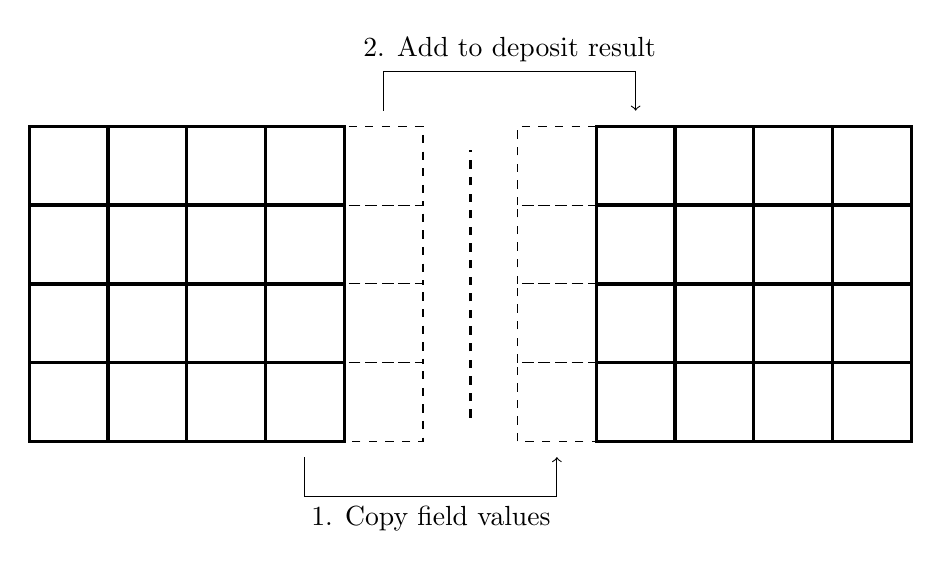
\begin{tikzpicture}
    \begin{scope}
      \foreach \y in {0,1,2,3} {
        \foreach \x in {0,1,2,3} {
          \draw[very thick] (\x, \y) rectangle (\x + 1, \y + 1);
        }
        \draw[dashed] (4,\y) rectangle (5,\y+1);
      }
    \end{scope}
    \begin{scope}[xshift=7.2cm]
      \foreach \y in {0,1,2,3} {
        \draw[dashed] (-1,\y) rectangle (0,\y+1);
        \foreach \x in {0,1,2,3} {
          \draw[very thick] (\x, \y) rectangle (\x + 1, \y + 1);
        }
      }
    \end{scope}
    \draw[->] (3.5, -0.2) -- (3.5, -0.7) -- node[midway,below] {1. Copy field values} (6.7, -0.7) -- (6.7, -0.2);
    \draw[->] (4.5, 4.2) -- (4.5, 4.7) -- node[midway,above] {2. Add to deposit result} (7.7, 4.7) -- (7.7, 4.2);
    \draw[dashed, very thick] (5.6, 0.3) -- (5.6, 3.7);
\end{tikzpicture}
  \caption[Guard cells between nodes.]{Guard cells between nodes. Two modes of
    inter-node communication. For field solver, the guard cells copies the values
  of the corresponding cells in the neighboring node (mode 1). For current
  deposition, the deposit results in the guard cells are added to the
  corresponding cells in the neighboring node (mode 2).}
  \label{fig:guard-cells}
\end{figure}

The CPU version of Aperture has been deployed on different platforms and shows
excellent scaling properties. It has been run on a local workstation with 12
cores, the Habanero cluster at Columbia on $\sim 250$ cores, and the NASA
Pleiades cluster on more than $10,000$ cores. The code can reliably achieve a
stable performance of $1.25$ million particles per core per second per timestep.
% (figure ).

% INSERT A PLOT SHOWING SCALING PROPERTIES

% Architecture of the code, each component is an independent class. Modularity.
% Special choices for GPU. Esirkepov deposit. High order shape functions and
% smoothness, vs performance penalty.

% Parallelization considerations. Performance.

% However, one of the challenges for achieving perfect scaling performance is load
% balancing between nodes. Since the performance is basically determined by the
% number of particles on the node, the node with the most particles is going to be
% slowest, and become the lowest common denominator for the whole simulation. In
% the problems that Aperture was designed to tackle, pair creation is an important
% feature, therefore it is very easy for some nodes to generate way more particles
% than others. Another factor is that due to spherical geometry and the way the
% grid is spaced uniformly in $\log r$ and $\theta$, cells further away from the
% star scale up in size as $r^{2}$ ($r^{3}$ in 3D). Therefore the nodes close to
% the outer boundary will be naturally more loaded.

\section{Test Problems}
\label{sec:test-problems}

In this section we present some well-known test cases to demonstrate the
correctness of the code. Due to the coordinate flexibility of Aperture, we would
like to test its correctness in multiple different coordinate systems. The
following three test cases are in Cartesian, cylindrical, and spherical
coordinates respectively, in the hope to represent the three main coordinate
systems that we support in the code.

\subsection{Relativistic Two-stream instability}
\label{sec:test-two-stream}

The first test is relativistic two-stream instability in 2D. We consider a
plasma beam with Lorentz factor of $\gamma_{b}$ and density $n_{b}$ passing
through a background with density $n_{p}$. The maximum growth rate of the
unstable mode is given by \citep[see e.g.][]{bret_collective_2004}:
\begin{equation}
  \label{eq:bret-2-stream}
  \delta_\mathrm{TSI} = \frac{\sqrt{3}}{2^{4/3}}\alpha^{1/3}/\gamma_{b}
\end{equation}
where $\alpha$ is the ratio of the number densities of the beam and background
$\alpha = n_{b}/n_{p}$.

\begin{figure}[h]
  \centering
  \includegraphics[width=0.7\textwidth]{pics/chap1/2stream.eps}
  \caption[Growth of two stream instability vs. theoretical value.]{Growth of
    two stream instability vs. theoretical value. Theoretical growth rate is
    $\delta_\mathrm{TSI}\approx 0.1375$ from equation \eqref{eq:bret-2-stream}.
    The growth saturates at around $t\omega_{p}\sim 130$.}
  \label{fig:test-2stream}
\end{figure}

We set up a neutral electron positron beam passing through a neutral electron
positron plasma background, with density ratio $\alpha = 1$ and initial beam
Lorentz factor $\gamma_{b} = 5.0$. We use a $512\times 256$ box with 512 cells
in the beam direction ($z$ direction in the $x$-$z$ plane), with roughly 5 cells
per plasma scale. We assume periodic boundary conditions on all boundaries.
Figure \ref{fig:test-2stream} shows the agreement of numerical growth of the
electric field energy with the prediction, up until saturation.

\subsection{Cylindrical Waveguide}
\label{sec:test-dispersion}

Consider a cylindrical waveguide with radius $r_{c}$ and periodic boundary
conditions at both ends, the system can be approximated as a long cylinder in
the limit of $\mathbf{B}_0\to \infty$, except with discretized $k_{z}$. The side
boundary of the cylinder is grounded, so $\Phi_{e} = 0$ at the boundary, which
also implies that $E_{\parallel} = 0$ on the boundary. With
these assumptions, the set of Maxwell equations can be solved analytically
\citep[see e.g.][]{swanson_plasma_2003}.
%(see e.g. Swanson 2003)
This calculation was also done in the context of pulsar flux tubes by
\citet{arons_wave_1986}, where they also discussed the $B \to \infty$ limit. We
repeat the calculation below and compare it with the numerical result obtained
in the simulation.

The radial solutions are lowest Bessel functions $J_0$ and
$J_1$, while the longitudinal solutions are simply plane waves:
\begin{subequations}
    \label{eqn:cyl-waveguide}
    \begin{align}
        E_z &= \sum_{n = 0}^\infty C_nJ_0(k_\perp r)e^{ik_zz - i\omega t} \\
        E_r &= \frac{ik_z}{\epsilon - k_z^2}\partial_r E_z = \sum_{n=0}^\infty \frac{ik_z k_\perp c^2}{\omega^2 - c^2k_z^2}C_nJ_1(k_\perp r)e^{ik_zz - i\omega t} \\
        B_\phi &= \frac{ic}{\omega}(\partial_r E_z - \partial_z E_r) = \sum_{n=0}^\infty \frac{i\omega c k_\perp}{\omega^2 - c^2k_z^2}C_n J_1(k_\perp r)e^{ik_zz - i\omega t} \\
        j_z &= \frac{i\omega_p^2}{4\pi \omega}E_z %= \sum_{n=0}^{\infty} \frac{i\omega_p^2}{4\pi \omega}C_n J_0(k_\perp r)e^{ik_zz - i\omega t}
    \end{align}
\end{subequations}
where $k_\perp$ is determined by the radial boundary condition that
$J_0(k_\perp r_\mathrm{c}) = 0$, and $n$ sums over the zeros of the
Bessel function. The fact that $E_z$ and $j_z$ are proportional to
$J_0$ while $B_\phi$ and $E_r$ are proportional to $J_1$ is determined
by our boundary condition that parallel electric field is zero at the
side of the cylinder. We have well-defined waves propagating along the
$z$ direction and the dispersion relation between $\omega$ and $k_z$
is:
\begin{equation}
    \left( \frac{\omega}{\omega_p} \right)^2 = \frac{1}{2}\left[ \left( 1 + k_\perp^2\lambda_p^2 + k_z^2\lambda_p^2 \right) \pm \sqrt{\left( 1 + k_\perp^2\lambda_p^2 + k_z^2\lambda_p^2 \right)^2 - 4k_z^2\lambda_p^2} \right]
    \label{eqn:disp_relation}
\end{equation}
This solution has two branches, as shown in figure~\ref{fig:disp_relation}.
\begin{figure}[h]
    \centering
    \begin{tikzpicture}[domain=0:3.5,smooth,scale=1.8]
        \draw[->,thick] (0,0) -- (4,0) node[below] {$k_z$};
        \draw[->,thick] (0,0) -- (0,4) node[left] {$\omega$};
        \draw plot[id=dispplot1] function{sqrt(0.5*(2 + x*x + sqrt((2 + x*x)*(2 + x*x) - 4*(x*x))))};
        \node [label=below:$E_z\gg B_{\phi}\,E_r$] at (3,1) {};
        \draw plot[id=dispplot2] function{sqrt(0.5*(2 + x*x - sqrt((2 + x*x)*(2 + x*x) - 4*(x*x))))};
        \node [label=above:$E_z\ll B_{\phi}\,E_r$] at (2.8,3.4) {};
        \node [label=left:$\sqrt{\omega_p^2 + c^2k_\perp^2}$] at (0,1.414) {};
        \draw[dashed] (0,0) -- (3.7,3.7) node[right] {$\omega/k_z = c$};
        \draw[dashed] (0,1) node[left] {$\omega_p$} -- (3.7,1);
        \draw[dashed] (0,0) -- (3.7,2.616) node[right] {$\displaystyle\omega/k_z = \frac{\omega_pc}{\sqrt{\omega_p^2 + c^2k_\perp^2}}$};
    \end{tikzpicture}
    \caption{Dispersion relation in the $B_z \to \infty$ limit}
    \label{fig:disp_relation}
\end{figure}
% The lower branch describes the Alfv\'en waves while the upper branch
% are electromagnetic waves.
For small $k$, the lower branch describes Alfv\'en waves, which correspond to
low-frequency oscillations of the magnetic field. The polarization vector is
dominated by $B_\phi$ and $E_r$. The upper branch represents Langmuir
oscillations whose polarization vector is dominated by $E_z$. For larger $k$,
the two branches change roles. The upper branch at higher $k$ corresponds to
ordinary EM waves with polarization vector along $E_r$ and phase speed close to
$c$, while the lower branch corresponds to plasma oscillations with frequency
approaching $\omega\sim \omega_p$.

Since $k_\perp$ determines the shape and positions of the two branches of the
dispersion relation, we need to select a particular $k_\perp$ in order to see a
well-defined dispersion curve. In order to accomplish this, we start with a
linear combination of normal modes with a wide range of $k_z$ that lie on both
branches and let them evolve in time. The initial state is composed from normal
mode exact solutions, so they should remain as normal modes after time
evolution. Periodic boundary condition is assumed at both lower and upper
boundaries. We used the 20th zero of the Bessel function $J_0$ to better
separate the two branches. The numerical dispersion relation is obtained by
taking the above initial condition and let it evolve for a light-crossing time
of the box. Then we take the real part of the 2D Fourier transform of the
electric field and magnetic field amplitude along a fixed $r$ as a function of
$z$ and $t$. The resolution is 1024 by 1024 with 10 cells in a single
$\lambda_p$ in the $z$ direction, and the time step is taken to be
$0.02\omega_p^{-1}$. Result is as shown in Figure~\ref{fig:disp_numerical}.
\begin{figure}[h]
    \centering
    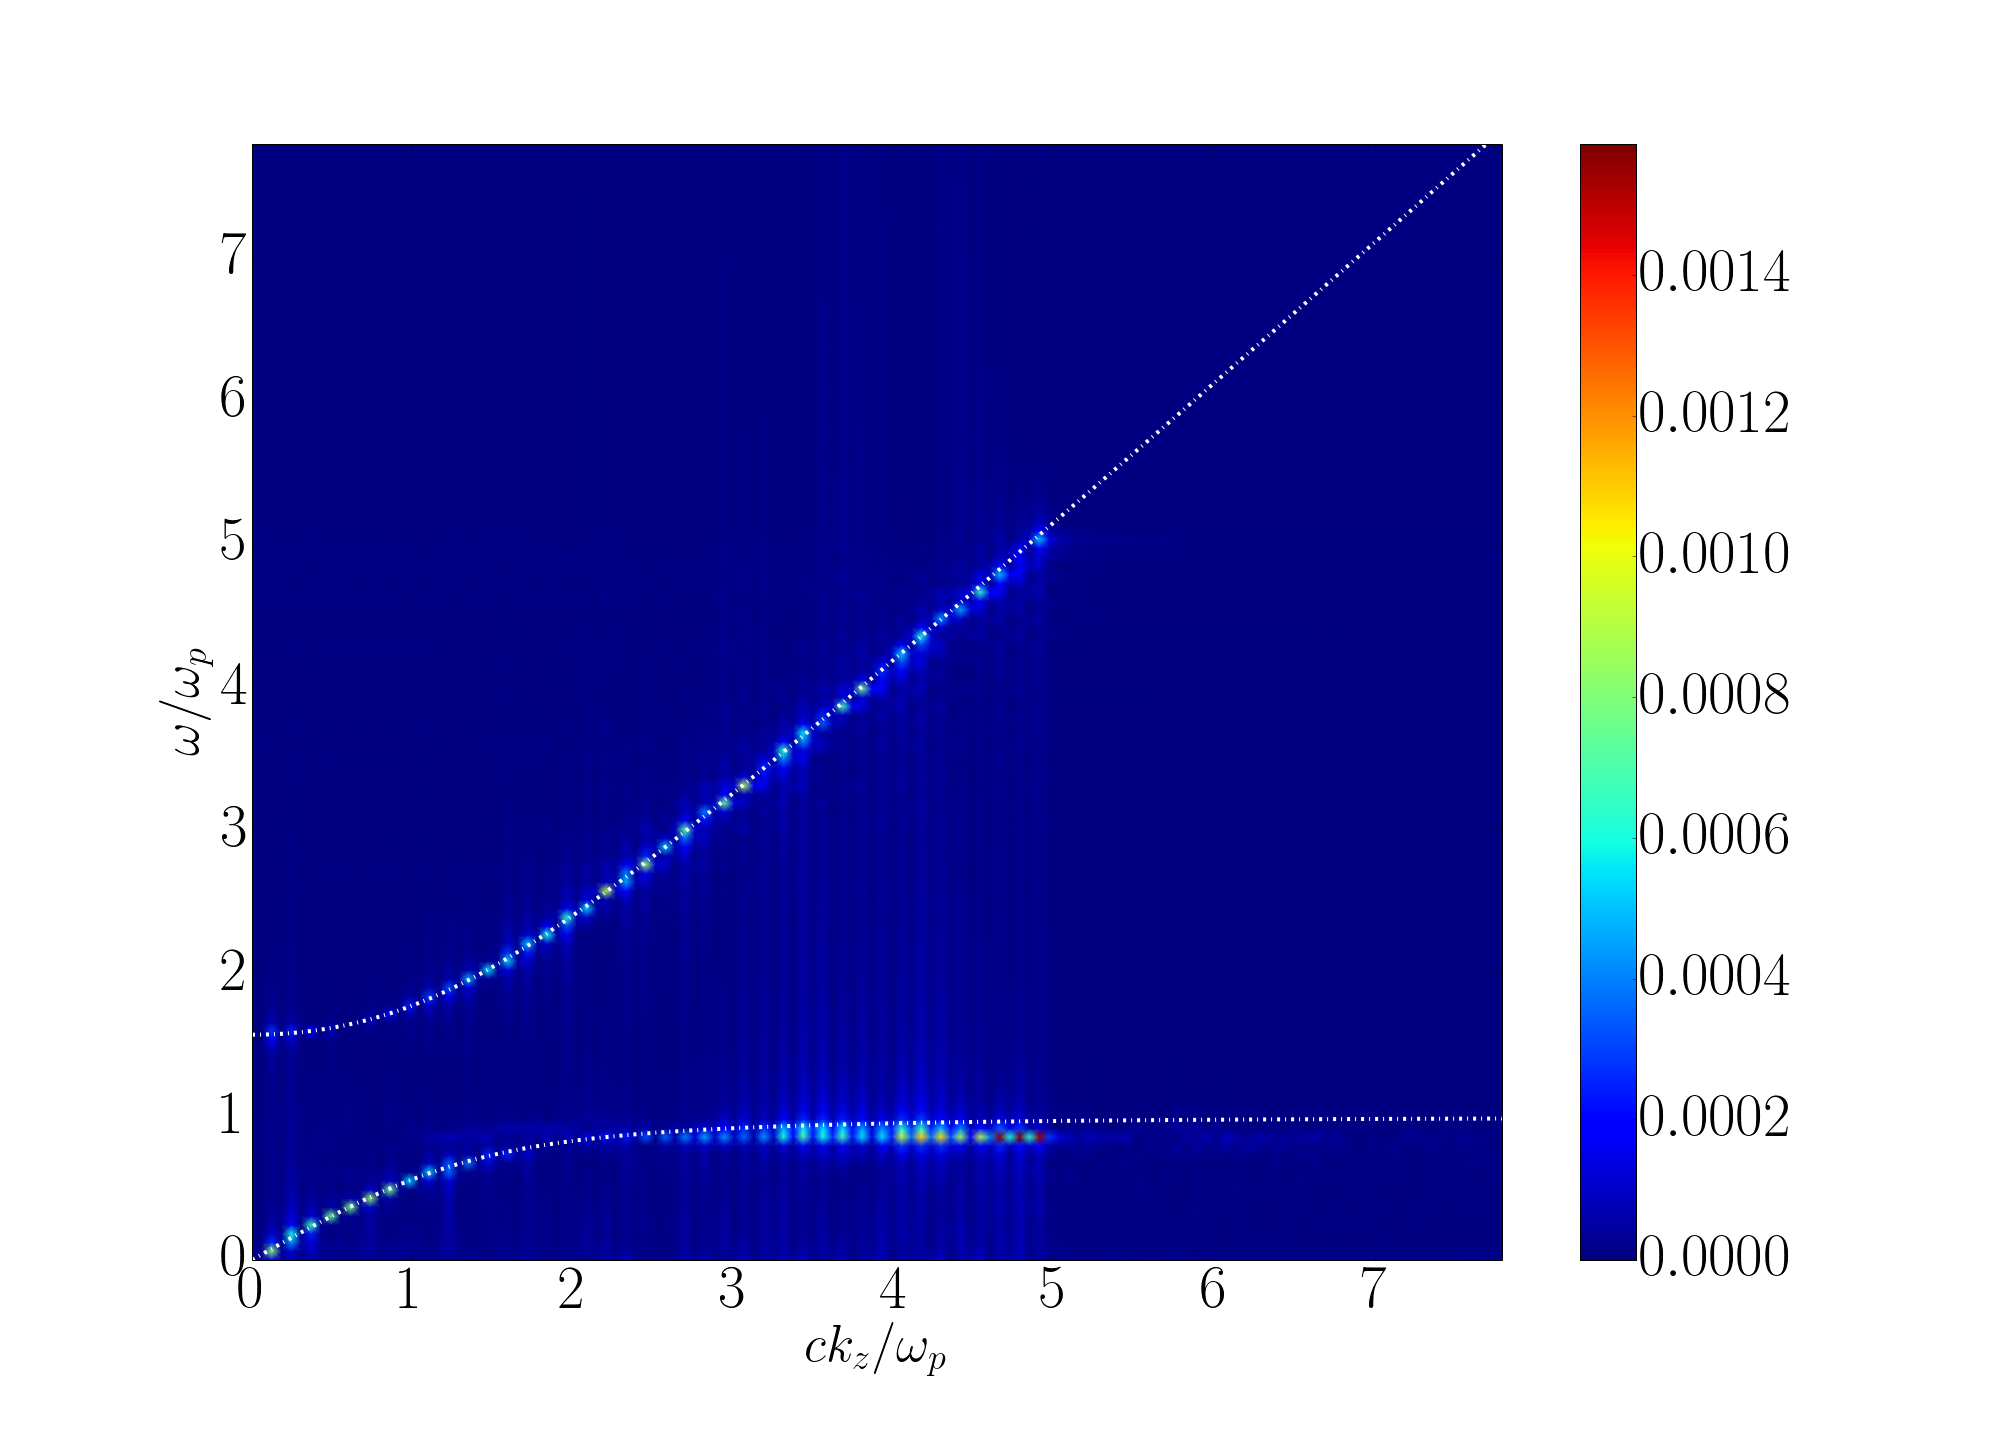
\includegraphics[width=0.8\textwidth]{pics/chap1/disp.png}
    \caption[Numerical dispersion relation for cylindrical waveguide.]{Numerical
      dispersion relation for a cylindrical waveguide. 2D plot shows the real
      part of the discrete Fourier transform of $E_z(z,t)$ at $r =
      1/4r_\mathrm{c}$. White dotted curve shows the theoretical dispersion
      relation calculated from Equation~ \eqref{eqn:disp_relation}.}
    \label{fig:disp_numerical}
\end{figure}

The lower branch of the numerical dispersion relation curves down with
respect to the theoretical line at high $k$. This is due to discretization on the
grid which creates an effective dispersion relation that deviates from
the theoretical one at small wavelengths. This can be seen simply from taking numerical derivatives of the simple solution $e^{ikx}$. The derivative, instead of $ike^{ikx}$, will look like
\begin{equation}
    \frac{e^{ik(x+\Delta x)} - e^{ik(x-\Delta x)}}{2\Delta x} = i\frac{\sin(k\Delta x)}{\Delta x} e^{ikx}
\end{equation}
This modifies the behavior of the dispersion relation when $k\Delta x \sim 1$,
and reduces the phase velocity of the waves at small wavelengths. It leads to
numerical Cherenkov radiation which is produced when particles travel faster
than the speed of the waves inside the medium. The wavelengths of this kind of
numerical radiation is always comparable to the grid scale, therefore can be
damped from the semi-implicit scheme we employed as described in
section~\ref{sec:fd-maxwell}. In practice, we do not observe strong sub-plasma
scale oscillations which are characteristic of numerical Cherenkov radiation.


\subsection{Monopole magnetosphere}
\label{sec:test-monopole}

\citet{michel_rotating_1973} found an analytic solution for the force-free
magnetosphere of a rotating magnetic monopole. The solution is such that the
toroidal field is proportional to the poloidal field:
\begin{equation}
  \label{eq:monopole-toroidal}
  B_{\phi} = -\frac{\Omega r\sin\theta}{c} B_{p}
\end{equation}
The corotating electric field defined by $\mathbf{E} =
-\mathbf{v}_\mathrm{rot}\times \mathbf{B}/c$ only has a $\theta$ component and it
is equal to $B_{\phi}$ in magnitude.

\begin{figure}[h]
  \centering
  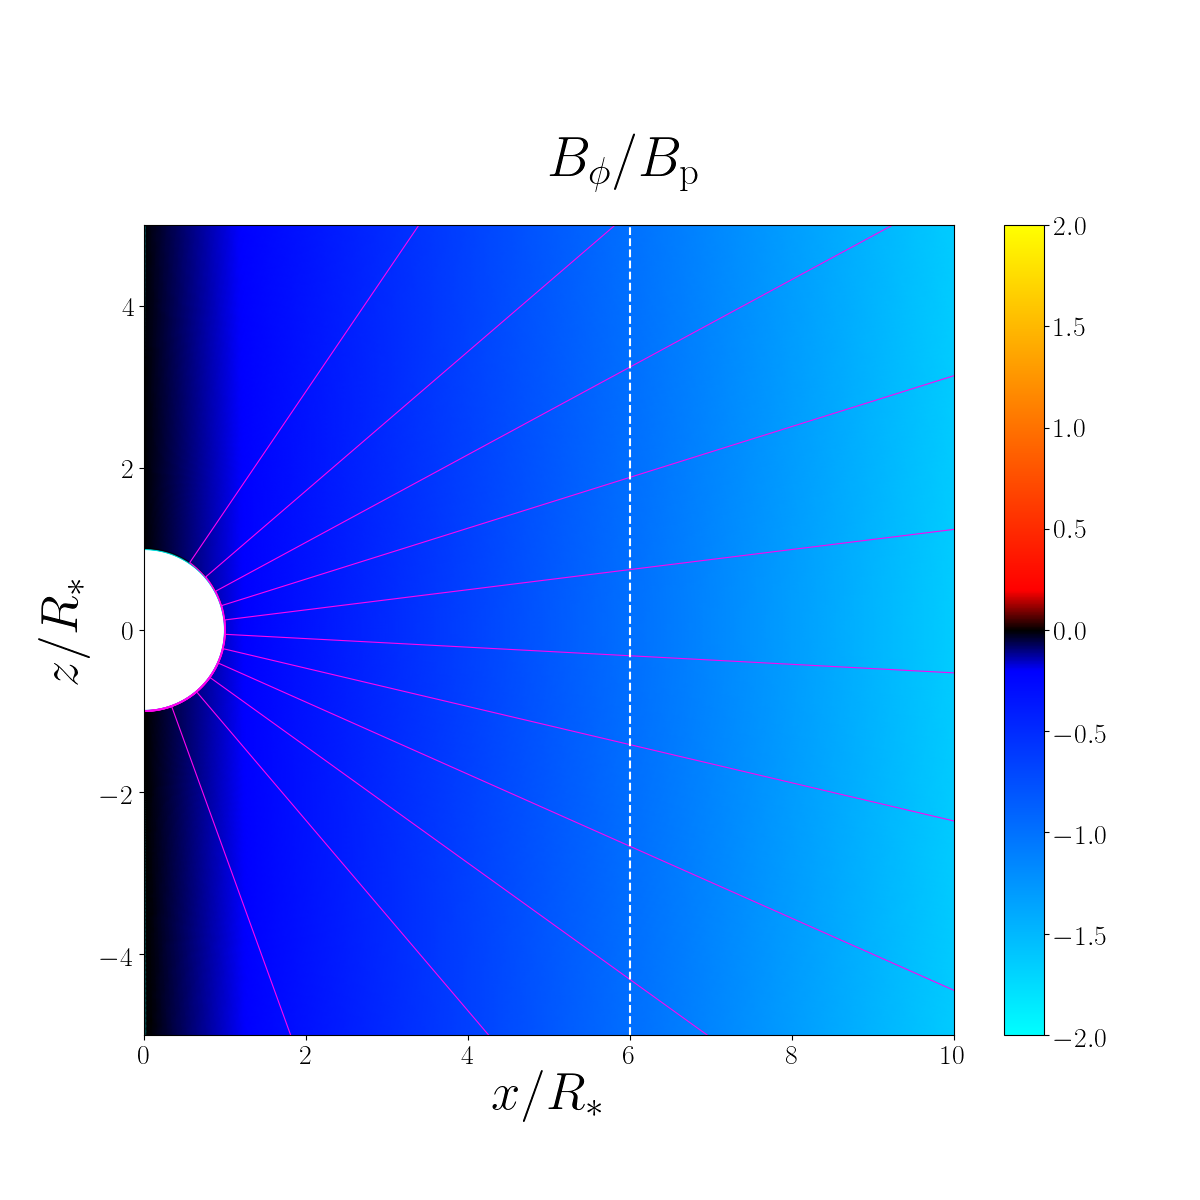
\includegraphics[width=0.6\textwidth]{pics/chap1/monopole-Bphi.png}
  \caption[Michel monopole solution.]{Michel monopole solution. Color shows the
    ratio of toroidal vs poloidal magnetic field $B_{\phi}/B_{p}$, which should
    be equal to $-\Omega r\sin\theta /c$. The ratio becomes -1 at the light
    cylinder, which is $r\sin\theta = 6R_{*}$ in this simulation, marked with
    a white dashed line. Purple lines are the poloidal field lines, which remain
    monopolar.}
  \label{fig:monopole-Bphi}
\end{figure}

We attempt to replicate this solution using PIC simulation. We found that field
configuration is identical to the analytic solution given above, with a
deviation near the stellar surface which consists of a parallel electric field
that accelerates particles to speed close to $c$. The simulation is run in
log-spherical coordinates with resolution $512\times 512$ in $\log r$ and
$\theta$. Figure \ref{fig:monopole-Bphi} shows the solution for $B_{\phi}$.

However, the magnetosphere cannot be force-free everywhere, as plasma is
injected at the stellar surface with velocity much smaller than $c$, and
particles have finite inertia. An acceleration process is needed to accelerate
the injected particles to speeds close to $c$. In a later paper by
\citet{michel_rotating_1974}, he derived the acceleration profile for the
space-charge limited flow, with terminal Lorentz factor $\gamma_{0}\to
\sigma^{1/2}$, where $\sigma$ is the magnetization defined as
$\omega_{B}R_{*}^2/\Omega R_\mathrm{LC}^2$. The particle acceleration is given
by the equation
\begin{equation}
  \label{eq:michel-accel}
  \frac{d}{dr}\left( r^2\frac{d\gamma}{dr} \right) - 2(\gamma - \gamma_0) = 2\sigma(\beta_0 - \beta)/\beta_0
\end{equation}
with an overall latitude dependence in the form of $\cos\theta$. Our simulation
shows also that $\gamma_0\sim \sigma^{1/2}$. In addition, the acceleration
profile follows the Michel solution as well (figure
\ref{fig:monopole-accel}). %TODO: add plot.

\begin{figure}[h]
  \centering
  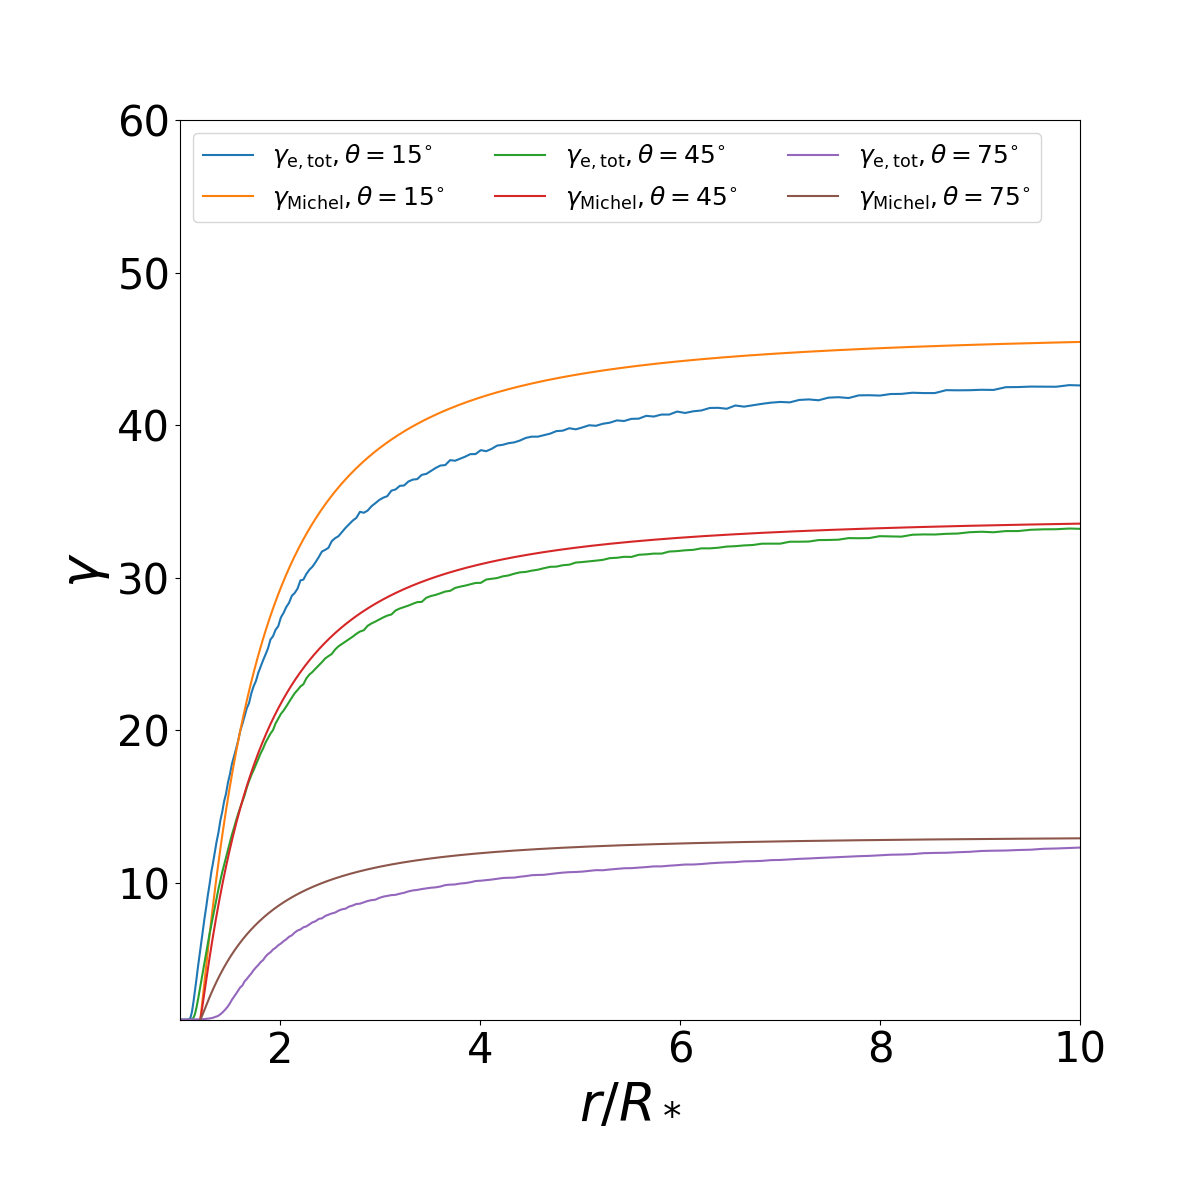
\includegraphics[width=0.6\textwidth]{pics/chap1/monopole-accel.png}
  \caption[Acceleration of charge-separated flow for a rotating magnetic
  monopole.]{Acceleration of charge-separated flow for a rotating magnetic
    monopole. The numerical curve matches the Michel solution fairly well,
    especially at $\theta = 45^{\circ}$.}
  \label{fig:monopole-accel}
\end{figure}

% This section we present some tests that show the validity of the
% code, in several coordinate systems, and in several physical scenarios

% \section{Example Applications}
% \label{sec:example-applications}
% This section we present some of toy physical models that we can
% simulate using this code, including axisymmetric pulsar (briefly),
% magnetar, twisted cylinder, Gruzinov problem, etc.

\section{Discussions and Remarks}
\label{sec:code-discussions}

We have explained the fundamentals of the Particle-in-Cell technique and the
design and structure of the Aperture code. Its novel features are support of
radiative transfer models and the built-in flexibility of cuvilinear
coordinates. The GPU version also enables the user to run medium-scale problems
relatively quickly on a small cost-efficient computer/cluster. In the following
chapters we will explore what can be done with this tool to further our
understanding of the magnetosphere of neutron stars.

Aperture is not the top performing code on the market at the moment of writing.
The VPIC code for example, can push 10 million particles per second per core.
Load balancing issue further exacerbates the performance problem, since pair
creation naturally leads to some domain patches having many more particles than
others, thus becoming the lowest denominator for speed. An extreme scenario
which arose in one of our simulations was that a handful of patches had more
than 80\% of the particles in the whole simulation box, in which case the
simulation slows down to a crawl while most of the nodes are almost idling
except for the few most loaded cores.

There is no universal way around this load balancing issue, since it is inherent
to all PIC codes. Some like TRISTAN-MP implements dynamic rescaling of domain
patches to shrink the loaded patches and grow the idling patches in hope of
balancing out, but it does not work well with extreme particle density contrast.
An approach that we implemented in Aperture is to annihilate $e^{\pm}$ pairs, getting
rid of excess electrons and positrons in pairs when the total number of
particles in a cell exceeds some limit. It helps dramatically with pulsar
simulations where the current sheet contains many more particles than the
surrounding.

With the help of Rui Hu, another hybrid parallelization scheme is being
implemented which reduce the total number of domain patches, but the particles
residing in those patches can by dynamically offloaded to other cores to process
the particle push and current deposition. Since particle number is the main
bottleneck, this scheme in theory can achieve near perfect parallel scaling, and
accelerate simulations like pulsar magnetosphere by a factor of 10 or more. A
complete vectorization of the code is also being developed, potentially can
increase the raw performance by a factor of 2 to 4.

With the treatment of radiative transfer, the Aperture code can be used not only
for magnetospheric problems but also for reconnection problems where plasma
interaction with the radiation field is important, e.g.\ in black hole corona.

% Local Variables:
% TeX-master: "../thesis"
% zotero-collection: #("16" 0 2 (name "Thesis"))
% End:
